\documentclass[12pt, a4paper]{report}

% ==============================================================================
% TYPOGRAPHY & ENCODING (Times New Roman, 12pt, 1.5 Line Spacing)
% ==============================================================================
\usepackage[T1]{fontenc}
\usepackage[utf8]{inputenc}
\usepackage{newtxtext,newtxmath} % Standard Times New Roman typography
\usepackage{microtype}
\usepackage{setspace}
\onehalfspacing

% ==============================================================================
% PAGE GEOMETRY (1 Inch on All Sides)
% ==============================================================================
\usepackage[
  a4paper,
  left=1.00in,
  right=1.00in,
  top=1.00in,
  bottom=1.00in,
  headheight=18pt,
  headsep=12pt,
  footskip=28pt
]{geometry}

% ==============================================================================
% SECTION & CHAPTER HEADINGS FORMATTING
% Main Heading: 16pt, Sub Heading: 14pt, Sub-sub Heading: 12pt
% ==============================================================================
\usepackage{titlesec}

% Chapter Heading: 16pt Bold Uppercase
\titleformat{\chapter}[hang]
  {\bfseries\fontsize{16}{20}\selectfont}
  {\thechapter.}{0.55em}{\MakeUppercase}
\titlespacing*{\chapter}{0pt}{0pt}{20pt}

% Section Heading (Sub Heading): 14pt Bold
\titleformat{\section}
  {\bfseries\fontsize{14}{18}\selectfont}
  {\thesection.}{0.55em}{}
\titlespacing*{\section}{0pt}{16pt}{8pt}

% Subsection Heading (Sub-sub Heading): 12pt Bold
\titleformat{\subsection}
  {\bfseries\fontsize{12}{16}\selectfont}
  {\thesubsection.}{0.55em}{}
\titlespacing*{\subsection}{0pt}{12pt}{6pt}

% Sub-subsection Heading: 12pt Italic/Bold
\titleformat{\subsubsection}
  {\bfseries\fontsize{12}{15}\selectfont}
  {\thesubsubsection.}{0.55em}{}
\titlespacing*{\subsubsection}{0pt}{10pt}{4pt}

% Simplify chapter headers to remove default "Chapter N" prefix
\makeatletter
\renewcommand{\@makechapterhead}[1]{%
  \vspace*{0pt}%
  {\parindent\z@ \raggedright \normalfont
    \bfseries\fontsize{16}{20}\selectfont
    \thechapter.\quad\MakeUppercase{#1}\par\nobreak
    \vskip 20pt}}
\makeatother

% ==============================================================================
% MACE BORDER SETUP (Single Rectangular Border Around Each Page)
% ==============================================================================
\usepackage{tikz}
\usepackage{eso-pic}
\AddToShipoutPictureBG{%
\begin{tikzpicture}[remember picture,overlay]
\draw[line width=1.0pt]
    ([xshift=0.35in,yshift=-0.35in]current page.north west)
    rectangle
    ([xshift=-0.35in,yshift=0.35in]current page.south east);
\end{tikzpicture}%
}

% ==============================================================================
% HEADER & FOOTER FORMATTING
% ==============================================================================
\usepackage{fancyhdr}
\newcommand{\ReportTitle}{ClauseIQ -- Machine Learning-Based Contract Clause Classification and Intelligent Search System}
\newcommand{\DepartmentName}{Department of Computer Applications, MACE}

\pagestyle{fancy}
\fancyhf{}
\fancyhead[R]{\small\ReportTitle}
\fancyfoot[L]{\small\DepartmentName}
\fancyfoot[R]{\small\thepage}
\renewcommand{\headrulewidth}{0.6pt}
\renewcommand{\footrulewidth}{0.6pt}

% Plain style for chapter-opening pages (maintains identical header & footer)
\fancypagestyle{plain}{%
  \fancyhf{}
  \fancyhead[R]{\small\ReportTitle}
  \fancyfoot[L]{\small\DepartmentName}
  \fancyfoot[R]{\small\thepage}
  \renewcommand{\headrulewidth}{0.6pt}
  \renewcommand{\footrulewidth}{0.6pt}
}

% ==============================================================================
% PARAGRAPH FORMATTING (Indentation & Spacing)
% ==============================================================================
\setlength{\parindent}{0pt}
\setlength{\parskip}{0.75em}
\usepackage{ragged2e}
\AtBeginDocument{\justifying}

% ==============================================================================
% TABLES, FIGURES & UTILITIES
% ==============================================================================
\usepackage{graphicx}
\graphicspath{{figures/}}
\usepackage{caption}
\captionsetup{
  font=small,
  labelfont=bf,
  justification=centering,
  singlelinecheck=true,
  skip=6pt
}
\usepackage{booktabs}
\usepackage{array}
\usepackage{tabularx}
\usepackage{longtable}
\usepackage{amsmath}
\usepackage{enumitem}
\setlist[itemize]{leftmargin=1.5em, itemsep=2pt, topsep=4pt}
\setlist[enumerate]{leftmargin=1.7em, itemsep=2pt, topsep=4pt}

% Hyperref & URLs
\usepackage{xurl}
\usepackage[
  colorlinks=true,
  linkcolor=black,
  citecolor=black,
  urlcolor=blue,
  pdfborder={0 0 0}
]{hyperref}

% ==============================================================================
% DOCUMENT BEGINS
% ==============================================================================
\begin{document}

% ------------------------------------------------------------------------------
% 1. TITLE PAGE (No Header, No Footer, No Page Number)
% ------------------------------------------------------------------------------
\begin{titlepage}
\thispagestyle{empty}
\begin{center}
    \vspace*{0.2in}
    
    {\bfseries\fontsize{18}{22}\selectfont CLAUSEIQ -- MACHINE LEARNING-BASED CONTRACT CLAUSE CLASSIFICATION AND INTELLIGENT SEARCH SYSTEM\par}
    
    \vspace{0.35in}
    
    {\fontsize{13}{16}\selectfont\textit{INTERIM PROJECT REPORT}\par}
    
    \vspace{0.15in}
    
    {\fontsize{12}{15}\selectfont Submitted in partial fulfillment of the requirements for the award of the Degree of\par}
    \vspace{0.08in}
    {\bfseries\fontsize{14}{17}\selectfont MASTER OF COMPUTER APPLICATIONS\par}
    
    \vspace{0.35in}
    
    {\fontsize{12}{15}\selectfont Submitted by\par}
    \vspace{0.08in}
    {\bfseries\fontsize{14}{17}\selectfont MOHAMMED FARHAN K\par}
    {\fontsize{12}{15}\selectfont (Reg. No: MAC25MCA-2042)\par}
    
    \vspace{0.35in}
    
    {\fontsize{12}{15}\selectfont Under the guidance of\par}
    \vspace{0.08in}
    {\bfseries\fontsize{13}{16}\selectfont Dr. SONIA ABRAHAM\par}
    {\fontsize{12}{15}\selectfont Associate Professor, Department of Computer Applications\par}
    
    \vspace{0.45in}
    
    {\bfseries\fontsize{13}{16}\selectfont DEPARTMENT OF COMPUTER APPLICATIONS\par}
    {\bfseries\fontsize{12}{15}\selectfont MAR ATHANASIUS COLLEGE OF ENGINEERING\par}
    {\fontsize{11}{14}\selectfont KOTHAMANGALAM, KERALA -- 686666\par}
    \vspace{0.08in}
    {\fontsize{12}{15}\selectfont SEPTEMBER 2026\par}
    
\end{center}
\end{titlepage}

% ------------------------------------------------------------------------------
% 2. CERTIFICATE (No Page Number)
% ------------------------------------------------------------------------------
\newpage
\thispagestyle{empty}
\begin{center}
    {\bfseries\fontsize{14}{17}\selectfont DEPARTMENT OF COMPUTER APPLICATIONS\par}
    {\bfseries\fontsize{13}{16}\selectfont MAR ATHANASIUS COLLEGE OF ENGINEERING\par}
    {\fontsize{11}{14}\selectfont KOTHAMANGALAM, KERALA -- 686666\par}
    
    \vspace{0.3in}
    
    {\bfseries\fontsize{16}{19}\selectfont\underline{BONAFIDE CERTIFICATE}\par}
\end{center}

\vspace{0.25in}

{\justifying\fontsize{12}{17}\selectfont
This is to certify that this interim project report titled \textbf{``ClauseIQ -- Machine Learning-Based Contract Clause Classification and Intelligent Search System''} is a bonafide record of the work carried out by \textbf{MOHAMMED FARHAN K} (Reg. No: \textbf{MAC25MCA-2042}) in partial fulfillment of the requirements for the award of the Degree of \textbf{Master of Computer Applications} from the \textbf{APJ Abdul Kalam Technological University} during the academic year 2025--2027.\par}

\vspace{0.6in}

\noindent
\begin{minipage}[t]{0.45\textwidth}
    \centering
    \textbf{Dr. SONIA ABRAHAM}\\
    Project Guide\\
    Associate Professor\\
    Department of Computer Applications\\
    MACE, Kothamangalam
\end{minipage}
\hfill
\begin{minipage}[t]{0.45\textwidth}
    \centering
    \textbf{MANU JOHN / MINU MARIA JOSEPH}\\
    Project Coordinators\\
    Assistant Professors\\
    Department of Computer Applications\\
    MACE, Kothamangalam
\end{minipage}

\vspace{0.8in}

\begin{center}
    \textbf{HEAD OF THE DEPARTMENT}\\
    Department of Computer Applications\\
    Mar Athanasius College of Engineering\\
    Kothamangalam, Kerala
\end{center}

% ------------------------------------------------------------------------------
% 3. DECLARATION (Starts Roman Page Numbering: Page i)
% ------------------------------------------------------------------------------
\newpage
\pagenumbering{roman}
\setcounter{page}{1}

\begin{center}
    {\bfseries\fontsize{16}{19}\selectfont DECLARATION\par}
\end{center}

\vspace{0.2in}

{\justifying\fontsize{12}{17}\selectfont
I, \textbf{MOHAMMED FARHAN K} (Reg. No: \textbf{MAC25MCA-2042}), hereby declare that the interim project report entitled \textbf{``ClauseIQ -- Machine Learning-Based Contract Clause Classification and Intelligent Search System''} submitted to the Department of Computer Applications, Mar Athanasius College of Engineering, Kothamangalam, in partial fulfillment of the requirements for the award of the Degree of \textbf{Master of Computer Applications}, is an authentic record of original work carried out by me under the guidance and supervision of \textbf{Dr. Sonia Abraham}, Associate Professor, Department of Computer Applications.

I further declare that this report has not previously formed the basis for the award of any degree, diploma, associateship, fellowship, or other similar title of recognition to any university or institution.\par}

\vspace{0.8in}

\noindent
\begin{minipage}[t]{0.5\textwidth}
    \textbf{Place:} Kothamangalam\\
    \textbf{Date:} 29-09-2026
\end{minipage}
\hfill
\begin{minipage}[t]{0.4\textwidth}
    \raggedleft
    \textbf{MOHAMMED FARHAN K}\\
    Reg. No: MAC25MCA-2042
\end{minipage}

% ------------------------------------------------------------------------------
% 4. ACKNOWLEDGEMENT (Page ii)
% ------------------------------------------------------------------------------
\newpage
\begin{center}
    {\bfseries\fontsize{16}{19}\selectfont ACKNOWLEDGEMENT\par}
\end{center}

\vspace{0.2in}

{\justifying\fontsize{12}{17}\selectfont
I take this opportunity to express my profound gratitude and heartfelt appreciation to all individuals who have contributed to the successful completion of this interim project phase.

First and foremost, I express my sincere gratitude to \textbf{Dr. Sonia Abraham}, Associate Professor and Project Guide, Department of Computer Applications, for her insightful guidance, valuable suggestions, constructive criticism, and continuous encouragement throughout the conception, modeling, and evaluation phases of ClauseIQ.

I extend my sincere thanks to \textbf{Prof. Manu John} and \textbf{Prof. Minu Maria Joseph}, Project Coordinators, for their meticulous scheduling, review assessments, and continuous support.

I express my deepest gratitude to the \textbf{Head of the Department}, Department of Computer Applications, and to the \textbf{Principal}, Mar Athanasius College of Engineering, Kothamangalam, for providing the state-of-the-art computational facilities and academic environment essential for conducting this research.

I also express my heartfelt thanks to all the faculty and non-teaching staff of the Department of Computer Applications for their direct and indirect assistance. Finally, I thank my family and friends for their enduring patience, encouragement, and support throughout the course of this work.\par}

\vspace{0.5in}
\begin{flushright}
    \textbf{MOHAMMED FARHAN K}
\end{flushright}

% ------------------------------------------------------------------------------
% 5. ABSTRACT (Page iii)
% ------------------------------------------------------------------------------
\newpage
\begin{center}
    {\bfseries\fontsize{16}{19}\selectfont ABSTRACT\par}
\end{center}

\vspace{0.2in}

{\justifying\fontsize{12}{17}\selectfont
Modern enterprises manage thousands of commercial contracts annually, where manual retrieval and categorization of operative clauses (such as limitation of liability, non-compete covenants, governing law, and audit rights) is labor-intensive, error-prone, and non-scalable. To address these industry bottlenecks, \textbf{ClauseIQ} is developed as a machine learning-based contract intelligence system that performs multi-class legal clause classification and intelligent semantic search.

ClauseIQ is built and evaluated upon the Contract Understanding Atticus Dataset (CUAD), an authoritative corpus of 510 commercial contracts curated from SEC EDGAR filings and expert-annotated across 41 legal clause categories. For this work, span annotations were flattened and cleaned into a structured tabular corpus of \textbf{12,204 clauses} spanning all \textbf{41 categories}. The dataset exhibits a severe real-world class imbalance ratio of \textbf{46.33 : 1}, ranging from 1,251 instances for \textit{Parties} to 27 instances for \textit{Price Restrictions}. Textual features are extracted using Term Frequency--Inverse Document Frequency (TF-IDF) configured for \textbf{10,000 unigram and bigram features} with sublinear term frequency scaling.

Four classical machine learning algorithms—Multinomial Naive Bayes, Linear Support Vector Machine (Linear SVM), Multinomial Logistic Regression, and Random Forest—were trained on a stratified 80\% split (\textbf{9,763 training samples}) and evaluated on an exact held-out 20\% split (\textbf{2,441 testing samples}) across all 41 categories. Hyperparameter tuning was conducted using Stratified K-Fold Cross-Validation optimizing explicitly for Macro-Averaged F1-Score (Macro-F1). 

On the held-out test set, \textbf{Logistic Regression} achieved \textbf{71.90\% Accuracy} and the highest \textbf{Macro-F1 of 64.74\%} (Weighted-F1: 71.96\%), while \textbf{Linear SVM} achieved \textbf{72.63\% Accuracy} and \textbf{64.18\% Macro-F1}. Because Macro-F1 weights all 41 categories equally under severe imbalance, and because Logistic Regression provides class probability estimates through its multinomial softmax formulation for confidence scoring, Logistic Regression was formally selected as the optimal production classifier. In parallel, a TF-IDF + Cosine Similarity search engine was developed and empirically benchmarked across canonical legal query scenarios, achieving a \textbf{Precision at 1 ($P@1$) of 80.00\%} and \textbf{Precision at 5 ($P@5$) of 88.00\%} with sub-10ms query execution speed. The classification and search services are exposed via a modular FastAPI REST backend validated by an automated test suite with \textbf{15 passed tests (100\% pass rate)}. Remaining deliverables—including live Supabase PostgreSQL database integration and a React.js web interface—are clearly delineated for the final project phase.\par}

% ------------------------------------------------------------------------------
% 6. LIST OF TABLES (Page iv)
% ------------------------------------------------------------------------------
\newpage
\phantomsection
\addcontentsline{toc}{chapter}{List of Tables}
\listoftables

% ------------------------------------------------------------------------------
% 7. LIST OF FIGURES (Page v)
% ------------------------------------------------------------------------------
\newpage
\phantomsection
\addcontentsline{toc}{chapter}{List of Figures}
\listoffigures

% ------------------------------------------------------------------------------
% 8. CONTENTS (No Page Number)
% ------------------------------------------------------------------------------
\newpage
\begingroup
\fancypagestyle{plain}{%
  \fancyhf{}%
  \fancyhead[R]{\small\ReportTitle}%
  \fancyfoot[L]{\small\DepartmentName}%
  \fancyfoot[R]{}% Suppress page number on TOC pages
  \renewcommand{\headrulewidth}{0.6pt}%
  \renewcommand{\footrulewidth}{0.6pt}%
}
\pagestyle{plain}
\setcounter{secnumdepth}{3}
\setcounter{tocdepth}{2}
\tableofcontents
\clearpage
\endgroup

% ------------------------------------------------------------------------------
% 9. MAIN BODY: CHAPTERS (Arabic Page Numbering Starts Here at Page 1)
% ------------------------------------------------------------------------------
\newpage
\pagenumbering{arabic}
\setcounter{page}{1}

\pagestyle{fancy}
\fancypagestyle{plain}{%
  \fancyhf{}%
  \fancyhead[R]{\small\ReportTitle}%
  \fancyfoot[L]{\small\DepartmentName}%
  \fancyfoot[R]{\small\thepage}%
  \renewcommand{\headrulewidth}{0.6pt}%
  \renewcommand{\footrulewidth}{0.6pt}%
}

\chapter{INTRODUCTION}
\label{ch:introduction}

\section*{Contract Review Problems in Modern Enterprises}
\label{sec:contract_problems}
Commercial contracts represent the legal, operational, and financial foundation of modern enterprise transactions. Within large organizations, procurement teams, legal departments, and corporate counsel execute and manage thousands of agreements annually, spanning non-disclosure agreements (NDAs), master service agreements (MSAs), software licenses, intellectual property assignments, and vendor contracts. 

Despite the critical nature of these legal instruments, contract review remains an overwhelmingly manual, resource-intensive, and error-prone process. Traditional contract triage requires attorneys and paralegals to spend dozens of hours manually reading dozens of pages per agreement to identify specific operative covenants, liabilities, and obligations. When an organization undergoes an audit, merger, or regulatory compliance review, teams must rapidly locate specific legal provisions—such as \textit{Cap on Liability}, \textit{Governing Law}, \textit{Termination for Convenience}, or \textit{Non-Compete} restrictions—across hundreds of disparate documents. Purely manual inspection does not scale: cognitive fatigue sets in, reviewers experience inconsistent interpretation across clauses, and high-risk terms are inadvertently overlooked.

\section*{Why Manual Clause Searching is Difficult}
\label{sec:manual_search_difficulties}
Locating specific clauses using legacy desktop search tools (such as standard word processing find tools or basic string matching) suffers from severe structural and linguistic limitations:
\begin{itemize}
    \item \textbf{Syntactic Variation:} Legal drafters employ widely different terminology to establish identical legal effects. For example, a limitation of liability provision may be phrased as ``\textit{aggregate liability shall not exceed the fees paid}'', ``\textit{under no circumstances shall either party be liable}'', or ``\textit{the sole and exclusive monetary remedy}''. Simple keyword matching fails to capture these semantically equivalent formulations.
    \item \textbf{Length and Complexity:} Legal provisions are frequently embedded within lengthy, multi-sentence paragraphs filled with conditional clauses, definitions, and cross-references. Locating the operative covenant requires isolating the specific clause boundaries from boilerplate preamble text.
    \item \textbf{Boilerplate Noise:} Standard provisions—such as notice requirements, severability, and counterpart execution clauses—often repeat across dozens of template agreements, creating search noise that distracts reviewers from bespoke commercial terms.
\end{itemize}

\section*{Importance of Legal NLP and Machine Learning}
\label{sec:importance_nlp_ml}
Natural Language Processing (NLP) and Machine Learning (ML) provide automated, data-driven solutions to overcome these manual bottlenecks. By transforming unstructured contract texts into mathematical representations, machine learning classifiers can automatically categorize clauses into standardized legal domains, while intelligent retrieval algorithms rank contract provisions based on query relevance.

Automating clause classification and search delivers substantial operational advantages:
\begin{enumerate}
    \item \textbf{Rapid Risk Identification:} Legal compliance teams can instantly isolate high-risk provisions (e.g., unlimited liability or restrictive non-compete covenants).
    \item \textbf{Consistency and Objectivity:} Algorithmic classification applies uniform categorization standards across all reviewed documents, eliminating human reviewer variability.
    \item \textbf{Significant Cost and Time Reduction:} Triage time is reduced from hours to seconds per document, allowing legal professionals to focus their attention on risk mitigation rather than rote reading.
\end{enumerate}

\section*{Why Classical Machine Learning is Chosen over Deep Learning or RAG}
\label{sec:classical_ml_justification}
While contemporary research frequently explores transformer architectures (e.g., Legal-BERT) and Large Language Models (LLMs) paired with Retrieval-Augmented Generation (RAG), this project deliberately implements and optimizes \textbf{classical machine learning algorithms} using Term Frequency--Inverse Document Frequency (TF-IDF) feature representations. This architectural decision is grounded in practical engineering, computational feasibility, and academic scope:
\begin{itemize}
    \item \textbf{Computational Efficiency and Hardware Constraints:} Deep learning and LLM pipelines require high-end GPU hardware for fine-tuning and inference. In contrast, classical classifiers (such as Logistic Regression, Linear Support Vector Machines, Multinomial Naive Bayes, and Random Forest) train in seconds to minutes on standard multi-core commodity CPUs and require minimal memory footprint.
    \item \textbf{Inference Latency:} Real-time enterprise contract search demands low-latency responses. In ClauseIQ, TF-IDF vectorization paired with Cosine Similarity executes clause similarity queries across more than 12,000 clauses in under 10 milliseconds, whereas generative LLM inference often introduces multi-second network and generation latency.
    \item \textbf{Determinism and Absence of Hallucinations:} In corporate compliance and legal due diligence, algorithmic hallucination is unacceptable. Generative models risk summarizing non-existent terms or misinterpreting statutory clauses. Classical classification and deterministic vector search return exact, verified clause text spans directly from the source contract.
    \item \textbf{Interpretability:} Linear models provide directly interpretable feature weights (term coefficients), enabling reviewers to verify exactly which legal vocabulary terms drove a classification decision.
    \item \textbf{Academic Mini-Project Scope:} As a Master of Computer Applications (MCA) semester mini project, establishing a rigorous, empirically tuned classical baseline provides an essential foundational benchmark before exploring complex neural systems.
\end{itemize}

\section*{Project Transition: From DocuMind AI to ClauseIQ}
\label{sec:project_transition}
During the initial project ideation phase, an exploratory proposal named ``DocuMind AI'' was conceptualized as a broad, multi-purpose document analysis system utilizing external generative APIs and RAG. However, detailed feasibility analysis and consultation with project guides revealed that relying on closed-source APIs lacked algorithmic rigor, introduced unpredictable API costs, raised data privacy concerns regarding confidential legal documents, and lacked reproducible empirical metrics.

Consequently, the project underwent a formal transition to \textbf{ClauseIQ: Machine Learning-Based Contract Clause Classification and Intelligent Search System}. Under ClauseIQ, the project scope was rigorously bounded to:
\begin{enumerate}
    \item Standardized supervised benchmark evaluation using the peer-reviewed Contract Understanding Atticus Dataset (CUAD).
    \item Full-scope 41-class legal categorization using four classical machine learning classifiers.
    \item End-to-end intelligent clause search utilizing vector similarity retrieval.
    \item Offline, self-contained architecture executing entirely on local infrastructure without external API dependencies.
\end{enumerate}

\section*{Introduction to the CUAD Benchmark}
\label{sec:cuad_intro}
ClauseIQ is trained and validated on the \textbf{Contract Understanding Atticus Dataset (CUAD)}, released by The Atticus Project and recognized by NeurIPS. CUAD comprises 510 real-world commercial contracts obtained from the U.S. Securities and Exchange Commission (SEC) EDGAR filing database. The dataset was exhaustively annotated by experienced legal professionals across 41 distinct legal clause categories, encompassing over 13,000 individually annotated text spans.

For the purpose of supervised machine learning and clause retrieval, CUAD's contract-level annotations were flattened and cleaned into a structured, tabular dataset consisting of \textbf{12,204 rows} across three primary columns: \texttt{contract\_id}, \texttt{clause\_text}, and \texttt{category}. Unlike simplified research projects that restrict classification to an arbitrary subset of 8 or 9 classes, ClauseIQ addresses the complete, unmodified \textbf{41-class categorization problem}, preserving the true real-world distribution and legal complexity of the domain.

\section*{Two Key Objectives of ClauseIQ}
\label{sec:two_key_objectives}
ClauseIQ addresses two complementary capabilities essential for contract intelligence:
\begin{enumerate}
    \item \textbf{Supervised Clause Classification:} Given an arbitrary clause extracted from a contract, automatically categorize it into one of the 41 CUAD legal categories (e.g., \textit{Audit Rights}, \textit{Governing Law}, \textit{Cap On Liability}) with an associated confidence score.
    \item \textbf{Intelligent Clause Search:} Given an ad-hoc natural language query from a reviewer (e.g., ``\textit{clauses limiting damages for breach}''), retrieve and rank the most semantically relevant clauses across the entire 12,204-clause corpus using TF-IDF representation and Cosine Similarity, supporting optional category-specific pre-filtering.
\end{enumerate}

\section*{Project Scope and Delimitations}
\label{sec:project_scope}
The scope of this interim project encompasses:
\begin{itemize}
    \item Complete exploratory data analysis and data validation of the flattened CUAD corpus.
    \item Robust text preprocessing, tokenization, stopword management, and 10,000-feature unigram+bigram TF-IDF vectorization with sublinear scaling.
    \item Systematic training, hyperparameter optimization, and empirical evaluation of four classical machine learning algorithms: Multinomial Naive Bayes, Linear Support Vector Machine, Logistic Regression, and Random Forest.
    \item Evaluation across all 41 categories on an exact, held-out 20\% test split ($N = 2,441$).
    \item Design and evaluation of a TF-IDF + Cosine Similarity intelligent search engine with retrieval precision and recall metrics ($P@k$ and $R@k$).
    \item Model serving via a modular FastAPI REST backend with automated test verification.
\end{itemize}

\textbf{Delimitations:} In accordance with the interim project boundaries, the user interface (React.js frontend), dynamic multi-page PDF ingestion pipeline, cloud deployment, and full Supabase PostgreSQL persistence are delineated as active or remaining work for the final phase.

\section*{Report Organization}
\label{sec:report_organization}
The remainder of this interim report is organized as follows:
\begin{itemize}
    \item \textbf{Chapter 2 (Supporting Literature):} Reviews existing literature in Legal NLP, text classification, and entity handling, summarizing foundational findings.
    \item \textbf{Chapter 3 (System Analysis):} Details exploratory data analysis, dataset distributions, class imbalance, text length statistics, mathematical formulation of algorithms, project pipeline, feasibility analysis, and system environment.
    \item \textbf{Chapter 4 (System Design):} Documents model building, implementation code, model planning (stratified 80/20 train/test splitting), training workflows, and testing procedures.
    \item \textbf{Chapter 5 (Results and Discussion):} Presents verified empirical model comparisons, evaluation metrics, confusion matrix analysis, relevant metrics calculated from the confusion matrix, prediction statistics of unseen data, and discussion of findings and conclusions.
\end{itemize}

\chapter{SUPPORTING LITERATURE}
\label{ch:supporting_literature}

\section{Literature Review}
\label{sec:literature_review}
To establish the theoretical and empirical grounding for ClauseIQ, this chapter reviews three foundational research publications in Legal Natural Language Processing (Legal NLP), contract analysis, and text classification published between 2023 and 2025 in \textit{IEEE Access}.

% ----------------------------------------------------------------------
% Paper 1
% ----------------------------------------------------------------------
\subsection*{Paper 1 -- Legal Natural Language Processing From 2015 to 2022: A Comprehensive Systematic Mapping Study of Advances and Applications}
\label{subsec:paper1}

\noindent\textbf{Authors:} Quevedo Caballero E., \v{C}ern\'{y} T., Rodriguez A., Rivas P., Yero J., Sooksatra K., Taibi D. \\
\textbf{Publication Details:} \textit{IEEE Access}, vol. 12, pp. 145286--145317, 2024. \\
\textbf{Digital Object Identifier (DOI):} \url{https://doi.org/10.1109/ACCESS.2024.3414967}

\subsubsection*{Overview and Area of Work}
This publication presents an exhaustive Systematic Mapping Study (SMS) of Legal NLP research published over an eight-year period (2015 to 2022). The authors systematically catalogued, classified, and analyzed 179 primary studies across digital libraries (IEEE Xplore, ACM Digital Library, Scopus, and Web of Science) to map the evolution of legal text processing tasks, algorithmic paradigms, benchmarks, and unresolved domain challenges.

\subsubsection*{Problem Statement and Scope}
Legal documents are characterized by domain-specific jargon, syntactic archaisms, non-linear cross-references, and structural variability that render general-purpose NLP models suboptimal. The study investigated what legal tasks are being automated, which datasets are establishing community benchmarks, and whether classical statistical models remain relevant alongside modern neural approaches.

\subsubsection*{Methodology}
The study followed established systematic literature review guidelines:
\begin{enumerate}
    \item Formulation of five targeted research questions focusing on task distribution, architectural choices, evaluation paradigms, and domain challenges.
    \item Rigorous multi-stage filtering from an initial corpus of over 2,400 papers down to 179 high-quality primary studies.
    \item Thematic taxonomy creation categorizing tasks into Information Extraction, Text Classification, Legal Information Retrieval, and Legal Judgment Prediction.
\end{enumerate}

\subsubsection*{Key Findings}
\begin{itemize}
    \item \textbf{Text Classification Prominence:} Multi-class legal document and clause classification emerged as one of the two most dominant task categories across the eight-year survey, accounting for nearly 30\% of all investigated literature.
    \item \textbf{Prevalence of Classical Baselines:} Despite the introduction of BERT and transformer models in 2018, classical machine learning approaches (particularly Support Vector Machines, Logistic Regression, and Naive Bayes coupled with n-gram TF-IDF representations) continue to serve as the universal standard baseline across more than 40\% of evaluated benchmarks.
    \item \textbf{Data Scarcity and Class Imbalance:} The authors identified extreme class imbalance and the scarcity of expert-annotated corpora as the single greatest bottleneck in real-world legal NLP deployment.
\end{itemize}

\subsubsection*{Relevance to ClauseIQ}
Quevedo Caballero et al. provide direct academic justification for ClauseIQ's architectural framework. Their survey validates that:
\begin{enumerate}
    \item Multi-class clause categorization is a core, legitimate problem in legal informatics.
    \item A classical TF-IDF baseline represents an essential, rigorous foundation before adopting more complex neural frameworks.
    \item Addressing severe class imbalance through specialized metrics (such as Macro-F1) is mandatory for credible legal classification systems.
\end{enumerate}

% ----------------------------------------------------------------------
% Paper 2
% ----------------------------------------------------------------------
\subsection*{Paper 2 -- Exploring LLMs Applications in Law: A Literature Review on Current Legal NLP Approaches}
\label{subsec:paper2}

\noindent\textbf{Authors:} Siino M., Falco M., Croce D., Rosso P. \\
\textbf{Publication Details:} \textit{IEEE Access}, vol. 13, pp. 18253--18276, 2025. \\
\textbf{Digital Object Identifier (DOI):} \url{https://doi.org/10.1109/ACCESS.2025.3533217}

\subsubsection*{Overview and Area of Work}
This survey examines the deployment of Large Language Models (LLMs) and advanced neural NLP techniques across diverse legal domains from 2017 through 2023, comparing them against classical and smaller fine-tuned models.

\subsubsection*{Problem Statement and Scope}
The rapid proliferation of generative language models has generated immense interest within legal technology. However, deploying multi-billion-parameter neural models introduces significant challenges, including hallucinations, high inference latency, prohibitive fine-tuning and hosting costs, lack of deterministic reproducibility, and data privacy concerns regarding confidential commercial contracts. This paper evaluates the practical trade-offs between classical NLP, specialized smaller models, and generative LLMs.

\subsubsection*{Methodology}
The authors conducted a PRISMA-compliant systematic review of 61 selected papers, synthesizing task performance, hardware footprints, dataset choices, and deployment feasibility across contract analysis, statutory interpretation, and legal document drafting.

\subsubsection*{Key Findings}
\begin{itemize}
    \item \textbf{CUAD as the Gold Standard:} The Contract Understanding Atticus Dataset (CUAD) was explicitly identified as the premier open-source benchmark for legal contract clause identification, cited across numerous experimental evaluations.
    \item \textbf{The Cost-Accuracy Trade-off:} The survey documented that while LLMs demonstrate strong zero-shot reasoning, carefully tuned classical algorithms and specialized discriminative models frequently achieve comparable or superior precision on narrowly scoped classification tasks, at a fraction of the computational and financial cost.
    \item \textbf{Real-World Deployment Barriers:} LLM-based solutions face severe latency barriers (often exceeding 2,000\,ms per query) and privacy liabilities when processing non-public contracts via cloud APIs, making local, lightweight pipelines highly attractive for practical enterprise adoption.
\end{itemize}

\subsubsection*{Relevance to ClauseIQ}
Siino et al.'s findings strongly corroborate ClauseIQ's technical choices:
\begin{enumerate}
    \item It directly validates the selection of CUAD as the premier benchmark for contract clause intelligence.
    \item It provides empirical support for a classical machine learning approach, demonstrating that high-cost generative LLMs are not inherently required for robust clause triage.
    \item It highlights the operational value of low-latency, deterministic, offline-capable architectures for legal workflows.
\end{enumerate}

% ----------------------------------------------------------------------
% Paper 3
% ----------------------------------------------------------------------
\subsection*{Paper 3 -- Named Entity Recognition Utilized to Enhance Text Classification While Preserving Privacy}
\label{subsec:paper3}

\noindent\textbf{Authors:} Kutbi M. \\
\textbf{Publication Details:} \textit{IEEE Access}, vol. 11, pp. 117576--117581, 2023. \\
\textbf{Digital Object Identifier (DOI):} \url{https://doi.org/10.1109/ACCESS.2023.3325895}

\subsubsection*{Overview and Area of Work}
Unlike the preceding systematic surveys, this publication is a targeted empirical research investigation. Kutbi explores whether applying Named Entity Recognition (NER) to identify and mask entity tokens (such as specific personal names, company names, and geographic locations) with standardized tags can improve downstream text classification accuracy while simultaneously protecting privacy in sensitive domain texts.

\subsubsection*{Problem Statement and Methodology}
In legal contracts, paragraphs frequently contain contract-specific proper nouns (e.g., specific counterparty names, monetary numbers, execution dates) that carry virtually zero discriminative signal for identifying the underlying clause category. Leaving raw named entities intact inflates the feature space with sparse, contract-specific tokens, causing overfitting and privacy leakage.

Kutbi evaluated a pipeline utilizing a spaCy NER model to detect named entities and replace them with generic placeholder tokens (e.g., \texttt{PERSON}, \texttt{ORG}, \texttt{GPE}) prior to TF-IDF feature extraction. The pipeline was tested on an in-house legal corpus of Limited Partnership Agreement (LPA) contract paragraphs (spanning 20 clause categories) alongside two benchmark general text datasets (Movie Reviews and Comparative Sentences). Classifiers including Linear Support Vector Machines were evaluated across unigram, bigram, and trigram configurations using 10 iterations of 5-fold cross-validation.

\subsubsection*{Key Experimental Results}
Kutbi reported original experimental results across feature configurations. Table \ref{tab:kutbi_results} reproduces the empirical findings on the legal Limited Partnership Agreement (LPA) dataset.

\begin{table}[h!]
\centering
\small
\begin{tabular}{lccc}
\toprule
\textbf{Dataset} & \textbf{N-gram Config} & \textbf{Linear SVM (Raw Text)} & \textbf{Linear SVM (+ NER Replacement)} \\
\midrule
Legal LPA (20 classes) & 1-gram & 55.37\% & 58.31\% \\
\textbf{Legal LPA (20 classes)} & \textbf{2-gram} & \textbf{55.60\%} & \textbf{63.76\%} \\
Legal LPA (20 classes) & 3-gram & 57.48\% & 62.83\% \\
\midrule
Movie Reviews & 1-gram & 81.00\% & 81.90\% \\
Movie Reviews & 2-gram & 82.50\% & 82.80\% \\
Movie Reviews & 3-gram & 82.60\% & 82.50\% \\
\midrule
Comparative Sentences & 1-gram & 68.30\% & 68.54\% \\
Comparative Sentences & 2-gram & 66.66\% & 67.37\% \\
Comparative Sentences & 3-gram & 65.25\% & 66.59\% \\
\bottomrule
\end{tabular}
\caption{Empirical evaluation of Linear SVM with and without entity replacement (Kutbi, 2023)}
\label{tab:kutbi_results}
\end{table}

The most significant finding for contract analysis is that on the legal LPA corpus, bigram (2-gram) Linear SVM classification accuracy improved substantially from \textbf{55.60\%} to \textbf{63.76\%} (an absolute gain of \textbf{+8.16\%}) when named entity replacement was introduced.

\subsubsection*{Relevance to ClauseIQ}
Kutbi's empirical investigation is directly relevant to ClauseIQ:
\begin{enumerate}
    \item It validates that classical Linear SVM models operating on n-gram TF-IDF representations are highly responsive to legal contract text classification.
    \item It demonstrates that bigram (2-gram) features yield superior discriminative capability over unigrams in legal contexts, directly supporting ClauseIQ's adoption of unigram+bigram TF-IDF feature extraction.
    \item It highlights that commercial contract clauses are laden with counterparty names and dates that can introduce feature noise, validating ClauseIQ's careful tokenization and stopword normalization.
\end{enumerate}

% ----------------------------------------------------------------------
% Section 2.2: Summary Table
% ----------------------------------------------------------------------
\section{Literature Review Summary}
\label{sec:literature_summary}
Table \ref{tab:lit_summary} synthesizes the core findings and architectural relevance of the three reviewed publications.

\begin{table}[h!]
\centering
\small
\begin{tabularx}{\textwidth}{p{2.8cm}p{3.2cm}p{4.2cm}X}
\toprule
\textbf{Publication} & \textbf{Approach / Scope} & \textbf{Key Findings} & \textbf{Relevance to ClauseIQ} \\
\midrule
\textbf{Quevedo Caballero et al. (2024)} \cite{quevedo2024} & 
Systematic Mapping Study of Legal NLP (2015--2022); 179 primary studies. & 
Multi-class text classification is a primary legal NLP task; classical TF-IDF baselines remain dominant; class imbalance is a major challenge. & 
Legitimizes classical TF-IDF classification for CUAD; reinforces the requirement for balanced/macro evaluation metrics. \\
\midrule
\textbf{Siino et al. (2025)} \cite{siino2025} & 
PRISMA review of LLMs and classical NLP in law (2017--2023); 61 papers. & 
Identifies CUAD as the standard benchmark; demonstrates that tuned classical models offer superior efficiency and deterministic output over LLMs. & 
Validates choice of CUAD benchmark; confirms computational, financial, and privacy benefits of classical ML. \\
\midrule
\textbf{Kutbi (2023)} \cite{kutbi2023} & 
Empirical evaluation on legal contract paragraphs using Linear SVM and NER. & 
Bigram representations paired with Linear SVM achieved 63.76\% accuracy on legal text; entity normalization reduces noise and improves accuracy. & 
Directly motivates unigram+bigram TF-IDF representations; provides comparative empirical baseline for legal clause classification. \\
\bottomrule
\end{tabularx}
\caption{Comprehensive summary of supporting literature}
\label{tab:lit_summary}
\end{table}

% ----------------------------------------------------------------------
% Section 2.3: Findings and Proposals
% ----------------------------------------------------------------------
\section{Findings and Proposals}
\label{sec:findings_and_proposals}
The synthesis of the supporting literature establishes three critical takeaways:
\begin{enumerate}
    \item \textbf{Domain Legitimacy:} Legal clause classification is an active, well-defined problem in applied computing with clear commercial utility.
    \item \textbf{Benchmark Authority:} CUAD is the literature-recognized, peer-reviewed standard for contract intelligence.
    \item \textbf{Classical ML Feasibility:} Classical machine learning algorithms operating on high-dimensional sparse TF-IDF vectors offer an optimal balance of accuracy, low latency, determinism, and computational thrift.
\end{enumerate}

\subsubsection*{Identified Research Gaps}
Despite the strengths of existing studies, significant practical gaps remain:
\begin{itemize}
    \item \textbf{Lack of Integrated Applications:} Most existing publications present isolated offline benchmark evaluations (e.g., reporting cross-validation numbers on static datasets) without delivering a deployable, interactive system that legal professionals can use.
    \item \textbf{Neglect of Retrieval:} Studies typically focus exclusively on classification or exclusively on search, whereas real-world contract triage requires both automated classification and free-text similarity search over the same clause index.
    \item \textbf{Arbitrary Class Down-sampling:} Many student and preliminary projects reduce CUAD to an arbitrary subset of 8 or 9 high-frequency categories, obscuring the severe real-world class imbalance across all 41 categories.
\end{itemize}

\subsubsection*{ClauseIQ System Proposals}
To directly bridge these identified gaps within an academically disciplined framework, ClauseIQ proposes:
\begin{enumerate}
    \item \textbf{Full 41-Category Classification:} Maintaining the complete, unpruned 41-class scope of the flattened CUAD corpus (12,204 rows), addressing the true 46.33:1 imbalance ratio.
    \item \textbf{Rigorous 4-Model Comparative Benchmark:} Implementing and systematically tuning four distinct classical algorithms (Logistic Regression, Linear SVM, Multinomial Naive Bayes, Random Forest) on an identical 80/20 held-out split.
    \item \textbf{Dual Capability (Classification + Intelligent Search):} Coupling multi-class classification with a TF-IDF + Cosine Similarity search engine over the exact same feature representation, evaluated empirically using Information Retrieval metrics ($P@k$ and $R@k$).
    \item \textbf{Modular API Architecture:} Wrapping model inference and search pipelines within a lightweight FastAPI REST backend to demonstrate end-to-end engineering completeness.
\end{enumerate}

\chapter{SYSTEM ANALYSIS}
\label{ch:system_analysis}

This chapter documents the empirical analysis of the dataset, data cleaning and preprocessing pipelines, exploratory data visualization, mathematical foundations of the proposed machine learning algorithms, end-to-end project pipeline, multidimensional feasibility study, and execution environment for ClauseIQ. All numerical metrics and distributions presented in this chapter are derived directly from the verified dataset and repository artifacts.

% ----------------------------------------------------------------------
% Section 3.1: Analysis of the Dataset
% ----------------------------------------------------------------------
\section{Analysis of the Dataset}
\label{sec:dataset_analysis}

\subsection{About the Dataset}
\label{subsec:about_dataset}
ClauseIQ is built upon the \textbf{Contract Understanding Atticus Dataset (CUAD)}, an authoritative legal natural language processing benchmark curated by The Atticus Project. CUAD consists of 510 real-world commercial contracts obtained from the United States Securities and Exchange Commission (SEC) EDGAR database. The corpus comprises diverse transactional agreements, including master services agreements, joint venture agreements, licensing pacts, intellectual property assignments, and merger documentation.

In its native distribution, CUAD is packaged in a SQuAD-style JSON format, wherein 41 distinct legal categories are mapped to span-level annotations across full contract documents. To construct a standardized, supervised classification and retrieval engine, these span annotations were extracted, normalized, and flattened into a structured tabular corpus.

The resulting working dataset of ClauseIQ contains \textbf{12,204 rows} structured into three core attributes:
\begin{enumerate}
    \item \texttt{contract\_id} (String): Unique identifier corresponding to the source commercial contract (510 unique contracts).
    \item \texttt{clause\_text} (String): The extracted, operative contractual text span.
    \item \texttt{category} (String): The expert-annotated legal category label (\textbf{41 unique classes}).
\end{enumerate}

Importantly, ClauseIQ models the full, unreduced \textbf{41-class problem space}. The system does not truncate the problem to an arbitrary subset of 8 or 9 classes, thereby preserving the genuine real-world taxonomy and difficulty of enterprise legal review.

\subsection{Explore the Dataset}
\label{subsec:explore_dataset}

\subsubsection*{Dataset Completeness and Missing Values}
Data integrity checks were executed across all 12,204 records in the flattened corpus. As summarized in Table \ref{tab:dataset_schema}, all three attributes exhibit 100\% completeness, with zero missing, null, or undefined values.

\begin{table}[h!]
\centering
\small
\begin{tabular}{lcccc}
\toprule
\textbf{Column Name} & \textbf{Data Type} & \textbf{Total Count} & \textbf{Missing Values} & \textbf{Completeness (\%)} \\
\midrule
\texttt{contract\_id} & String (Categorical) & 12,204 & 0 & 100.0\% \\
\texttt{clause\_text} & String (Text)        & 12,204 & 0 & 100.0\% \\
\texttt{category}    & String (Target)      & 12,204 & 0 & 100.0\% \\
\bottomrule
\end{tabular}
\caption{Dataset schema and missing value analysis ($N = 12,204$)}
\label{tab:dataset_schema}
\end{table}

\subsubsection*{Duplicate and Boilerplate Analysis}
Deduplication analysis revealed zero duplicate rows across the entire dataset. However, text-level analysis identified that \textbf{1,655 clause texts repeat across distinct contracts}, representing 13.56\% of all records, leaving \textbf{10,549 unique distinct clause text strings}. 

In legal contracting, this repetition is an expected domain characteristic rather than an artifact of faulty data collection. Commercial contracts heavily utilize standardized boilerplate covenants (e.g., standard ``\textit{prior written consent}'' stipulations, standard Delaware governing law provisions, or formal notice requirements) across unrelated corporate agreements. Preserving these shared boilerplate provisions is necessary to ensure the classifier learns standard legal phrasing.

\subsubsection*{Contract-Level Clause Distribution}
The 12,204 clauses originate from 510 distinct contracts. The distribution of clauses per contract varies significantly depending on contract complexity, governing structure, and total length:
\begin{itemize}
    \item \textbf{Mean clauses per contract:} 23.93
    \item \textbf{Median clauses per contract:} 19.00
    \item \textbf{Minimum clauses in a contract:} 1
    \item \textbf{Maximum clauses in a contract:} 93
\end{itemize}

Figure \ref{fig:clauses_per_contract} illustrates the distribution of clause counts per contract. While a typical agreement contains between 15 and 30 annotated clauses, complex transaction agreements contain up to 93 distinct provisions.

\begin{figure}[h!]
\centering
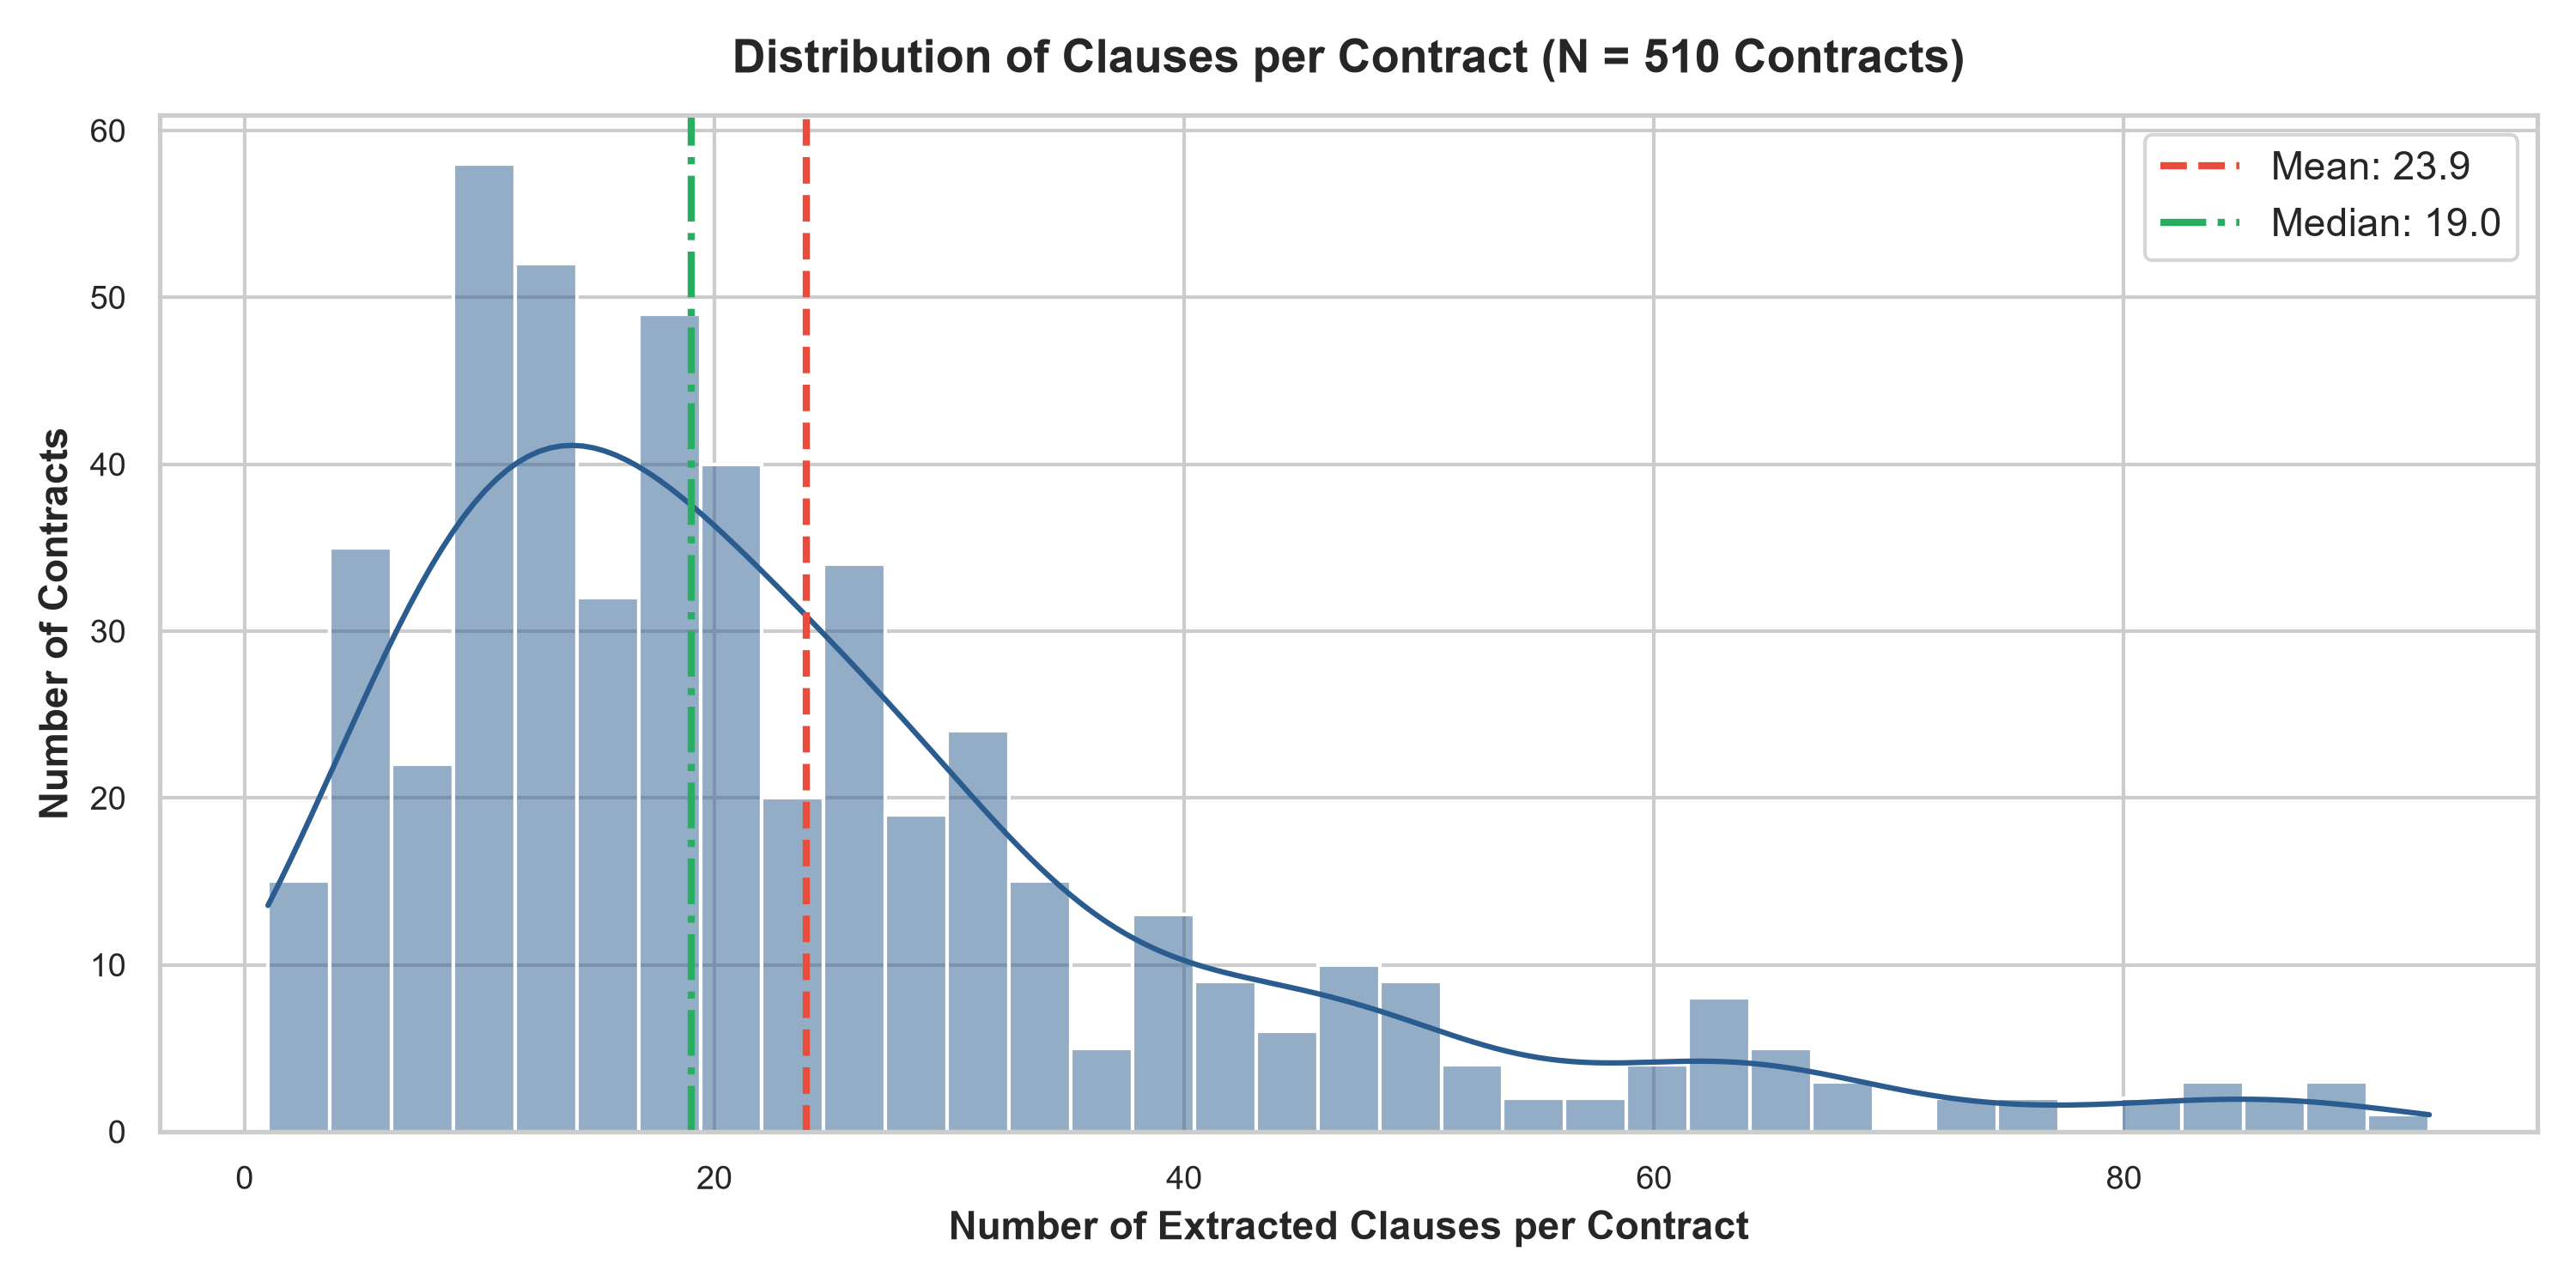
\includegraphics[width=0.85\textwidth]{figures/clauses_per_contract.png}
\caption{Distribution of annotated clauses per contract across 510 CUAD contracts}
\label{fig:clauses_per_contract}
\end{figure}

\subsubsection*{Class Distribution and Severe Imbalance}
The 41 legal categories display extreme class imbalance. Table \ref{tab:class_distribution_extremes} outlines the ten most frequent and five least frequent categories in the dataset.

\begin{table}[h!]
\centering
\small
\begin{tabular}{clcclc}
\toprule
\textbf{Rank} & \textbf{Category (Frequent)} & \textbf{Count} & \textbf{Rank} & \textbf{Category (Rare)} & \textbf{Count} \\
\midrule
1  & Parties                    & 1,251 & 37 & Source Code Escrow         & 67 \\
2  & Cap On Liability           & 742   & 38 & Unlimited/All-You-Can-Eat  & 43 \\
3  & Audit Rights               & 642   & 39 & Non-Disparagement          & 42 \\
4  & Governing Law              & 462   & 40 & Third Party Beneficiary    & 39 \\
5  & Anti-Assignment            & 652   & 41 & Price Restrictions         & 27 \\
\bottomrule
\end{tabular}
\caption{Most frequent vs. least frequent clause categories in ClauseIQ}
\label{tab:class_distribution_extremes}
\end{table}

The largest class, \textit{Parties}, comprises \textbf{1,251 clauses} (10.25\% of the total dataset), whereas the smallest category, \textit{Price Restrictions}, comprises merely \textbf{27 clauses} (0.22\% of the dataset). This establishes an extreme \textbf{class imbalance ratio of 46.33 : 1}. Section \ref{subsec:class_variables} addresses the critical algorithmic and evaluation implications of this distribution.

\subsubsection*{Text Length and Syntactic Statistics}
To quantify the linguistic characteristics of the clauses, three metrics were computed: word count, character length, and sentence count. Table \ref{tab:text_statistics} presents the summary statistics.

\begin{table}[h!]
\centering
\small
\begin{tabular}{lccc}
\toprule
\textbf{Metric} & \textbf{Word Count} & \textbf{Character Length} & \textbf{Sentence Count} \\
\midrule
\textbf{Minimum} & 3      & 9        & 1    \\
\textbf{Maximum} & 479    & 3,169    & 24   \\
\textbf{Mean}    & 45.89  & 289.16   & 1.48 \\
\textbf{Median}  & 36.00  & 228.00   & 1.00 \\
\textbf{Std Dev} & 39.42  & 251.84   & 1.12 \\
\bottomrule
\end{tabular}
\caption{Summary statistics of clause text dimensions ($N = 12,204$)}
\label{tab:text_statistics}
\end{table}

The statistics highlight substantial structural heterogeneity. The shortest valid clauses contain as few as 3 words (e.g., party entities or agreement dates), while expansive indemnification or non-compete clauses span up to 479 words and 24 sentences.

% ----------------------------------------------------------------------
% Section 3.2: Data Preprocessing
% ----------------------------------------------------------------------
\section{Data Preprocessing}
\label{sec:data_preprocessing}

\subsection{Data Cleaning}
\label{subsec:data_cleaning}
To transform raw contractual text into uniform numerical representations suitable for machine learning, a systematic preprocessing pipeline was implemented:
\begin{enumerate}
    \item \textbf{Text Extraction:} Ingestion of contractual text strings from structured CSV and document extractors.
    \item \textbf{Clause Splitting:} Detection of clause boundaries based on paragraph breaks, numbered section headers (e.g., \textit{Section 12.1}, \textit{Article IV}), and terminal punctuation.
    \item \textbf{Case Normalization:} Conversion of all text to lowercase to unify vocabulary (e.g., ``\textit{Shall}'' and ``\textit{shall}'' map to the same token).
    \item \textbf{Special Character and Punctuation Handling:} Removal of extraneous formatting characters (tabs, repeated hyphens, non-ASCII symbols) while preserving standard syntactical punctuation that delineates clauses.
    \item \textbf{Whitespace Consolidation:} Regex-based collapse of irregular whitespace into single space characters.
    \item \textbf{Tokenization and Stopword Filtering:} Word-level tokenization combined with English stopword filtering to eliminate low-information grammatical words without discarding legal connectors.
\end{enumerate}

\subsubsection*{Short-Clause and Long-Clause Preservation Policy}
A critical finding from exploratory data analysis is that \textbf{short clauses are not noise}. Legal contracts inherently contain concise, high-value provisions. For instance, in the CUAD dataset, metadata categories such as \textit{Parties} (mean length: 5.6 words) and \textit{Document Name} (mean length: 4.8 words) frequently contain fewer than 5 words. An automated filter removing spans under 5 words would eliminate \textbf{89.8\% of all Parties records} and \textbf{55.0\% of Document Name records}, severely damaging model training. 

Conversely, long clauses (reaching up to 479 words) represent comprehensive, highly negotiated covenants (e.g., complex \textit{Non-Compete} or \textit{License Grant} terms). Truncating these provisions would strip out essential restrictive qualifications. Therefore, all valid annotated clauses are retained, and \textbf{sublinear term frequency scaling} is introduced during vectorization to mathematically regulate the influence of very long provisions.

\subsection{Analysis of Feature Variables}
\label{subsec:feature_variables}
The primary feature variable is the raw \texttt{clause\_text}. While metadata metrics (word count, character length, sentence count) were engineered during EDA to understand the corpus, they are deliberately excluded from classifier training. Passing clause length as an explicit feature would introduce spurious correlations, as length alone cannot reliably differentiate legal rights.

Textual features are extracted using \textbf{Term Frequency--Inverse Document Frequency (TF-IDF)} with the following verified hyperparameters:
\begin{itemize}
    \item \textbf{Vocabulary Dimension:} Capped at the top \textbf{10,000 features} based on term frequency across the training split.
    \item \textbf{N-gram Range:} $(1, 2)$, capturing both unigrams (individual words) and bigrams (two-word collocations). In legal drafting, compound phrases such as ``\textit{governing law}'', ``\textit{prior written}'', and ``\textit{sole discretion}'' carry distinct legal meaning that individual unigrams cannot convey.
    \item \textbf{Sublinear TF Scaling:} Enabled ($\text{sublinear\_tf} = \text{True}$), replacing raw term frequency $TF$ with $1 + \log(TF)$, preventing long clauses with repetitive words from dominating vector magnitudes.
    \item \textbf{Document Frequency Bounds:} Terms appearing in fewer than 2 documents are excluded to filter out typographical anomalies.
\end{itemize}

\subsection{Analysis of Class Variables}
\label{subsec:class_variables}
The target variable is \texttt{category}, comprising 41 discrete legal classes. In a multi-class dataset exhibiting a 46.33:1 imbalance ratio, standard classification accuracy is a deceptive metric. A naive baseline that uniformly predicts the majority class (\textit{Parties}) would achieve an accuracy score while failing completely to detect critical risk categories such as \textit{Price Restrictions}, \textit{Most Favored Nation}, or \textit{Source Code Escrow}.

To ensure that rare categories receive equal optimization priority during model selection, the project adopts \textbf{Macro-Averaged F1-Score (Macro-F1)} as the primary evaluation metric:
\begin{equation}
    \text{Macro-F1} = \frac{1}{C} \sum_{c=1}^{C} F1_c
\end{equation}
where $C = 41$. Macro-F1 calculates the harmonic mean of precision and recall for each category independently and then computes their unweighted arithmetic mean. Under this formulation, correctly classifying a rare \textit{Price Restrictions} clause is weighted identically to classifying a frequent \textit{Parties} clause. Furthermore, class weighting ($\text{class\_weight} = \text{'balanced'}$) is applied to penalize misclassifications in minority classes proportionally to their inverse class frequencies.

% ----------------------------------------------------------------------
% Section 3.3: Data Visualization
% ----------------------------------------------------------------------
\section{Data Visualization}
\label{sec:data_visualization}

\subsection{Category Frequency Distribution}
Figure \ref{fig:class_distribution} displays the frequency distribution across all 41 legal categories in the ClauseIQ dataset. The extreme long-tail distribution visually confirms the severe imbalance, with the top 5 categories accounting for more than 30\% of the entire corpus.

\begin{figure}[h!]
\centering
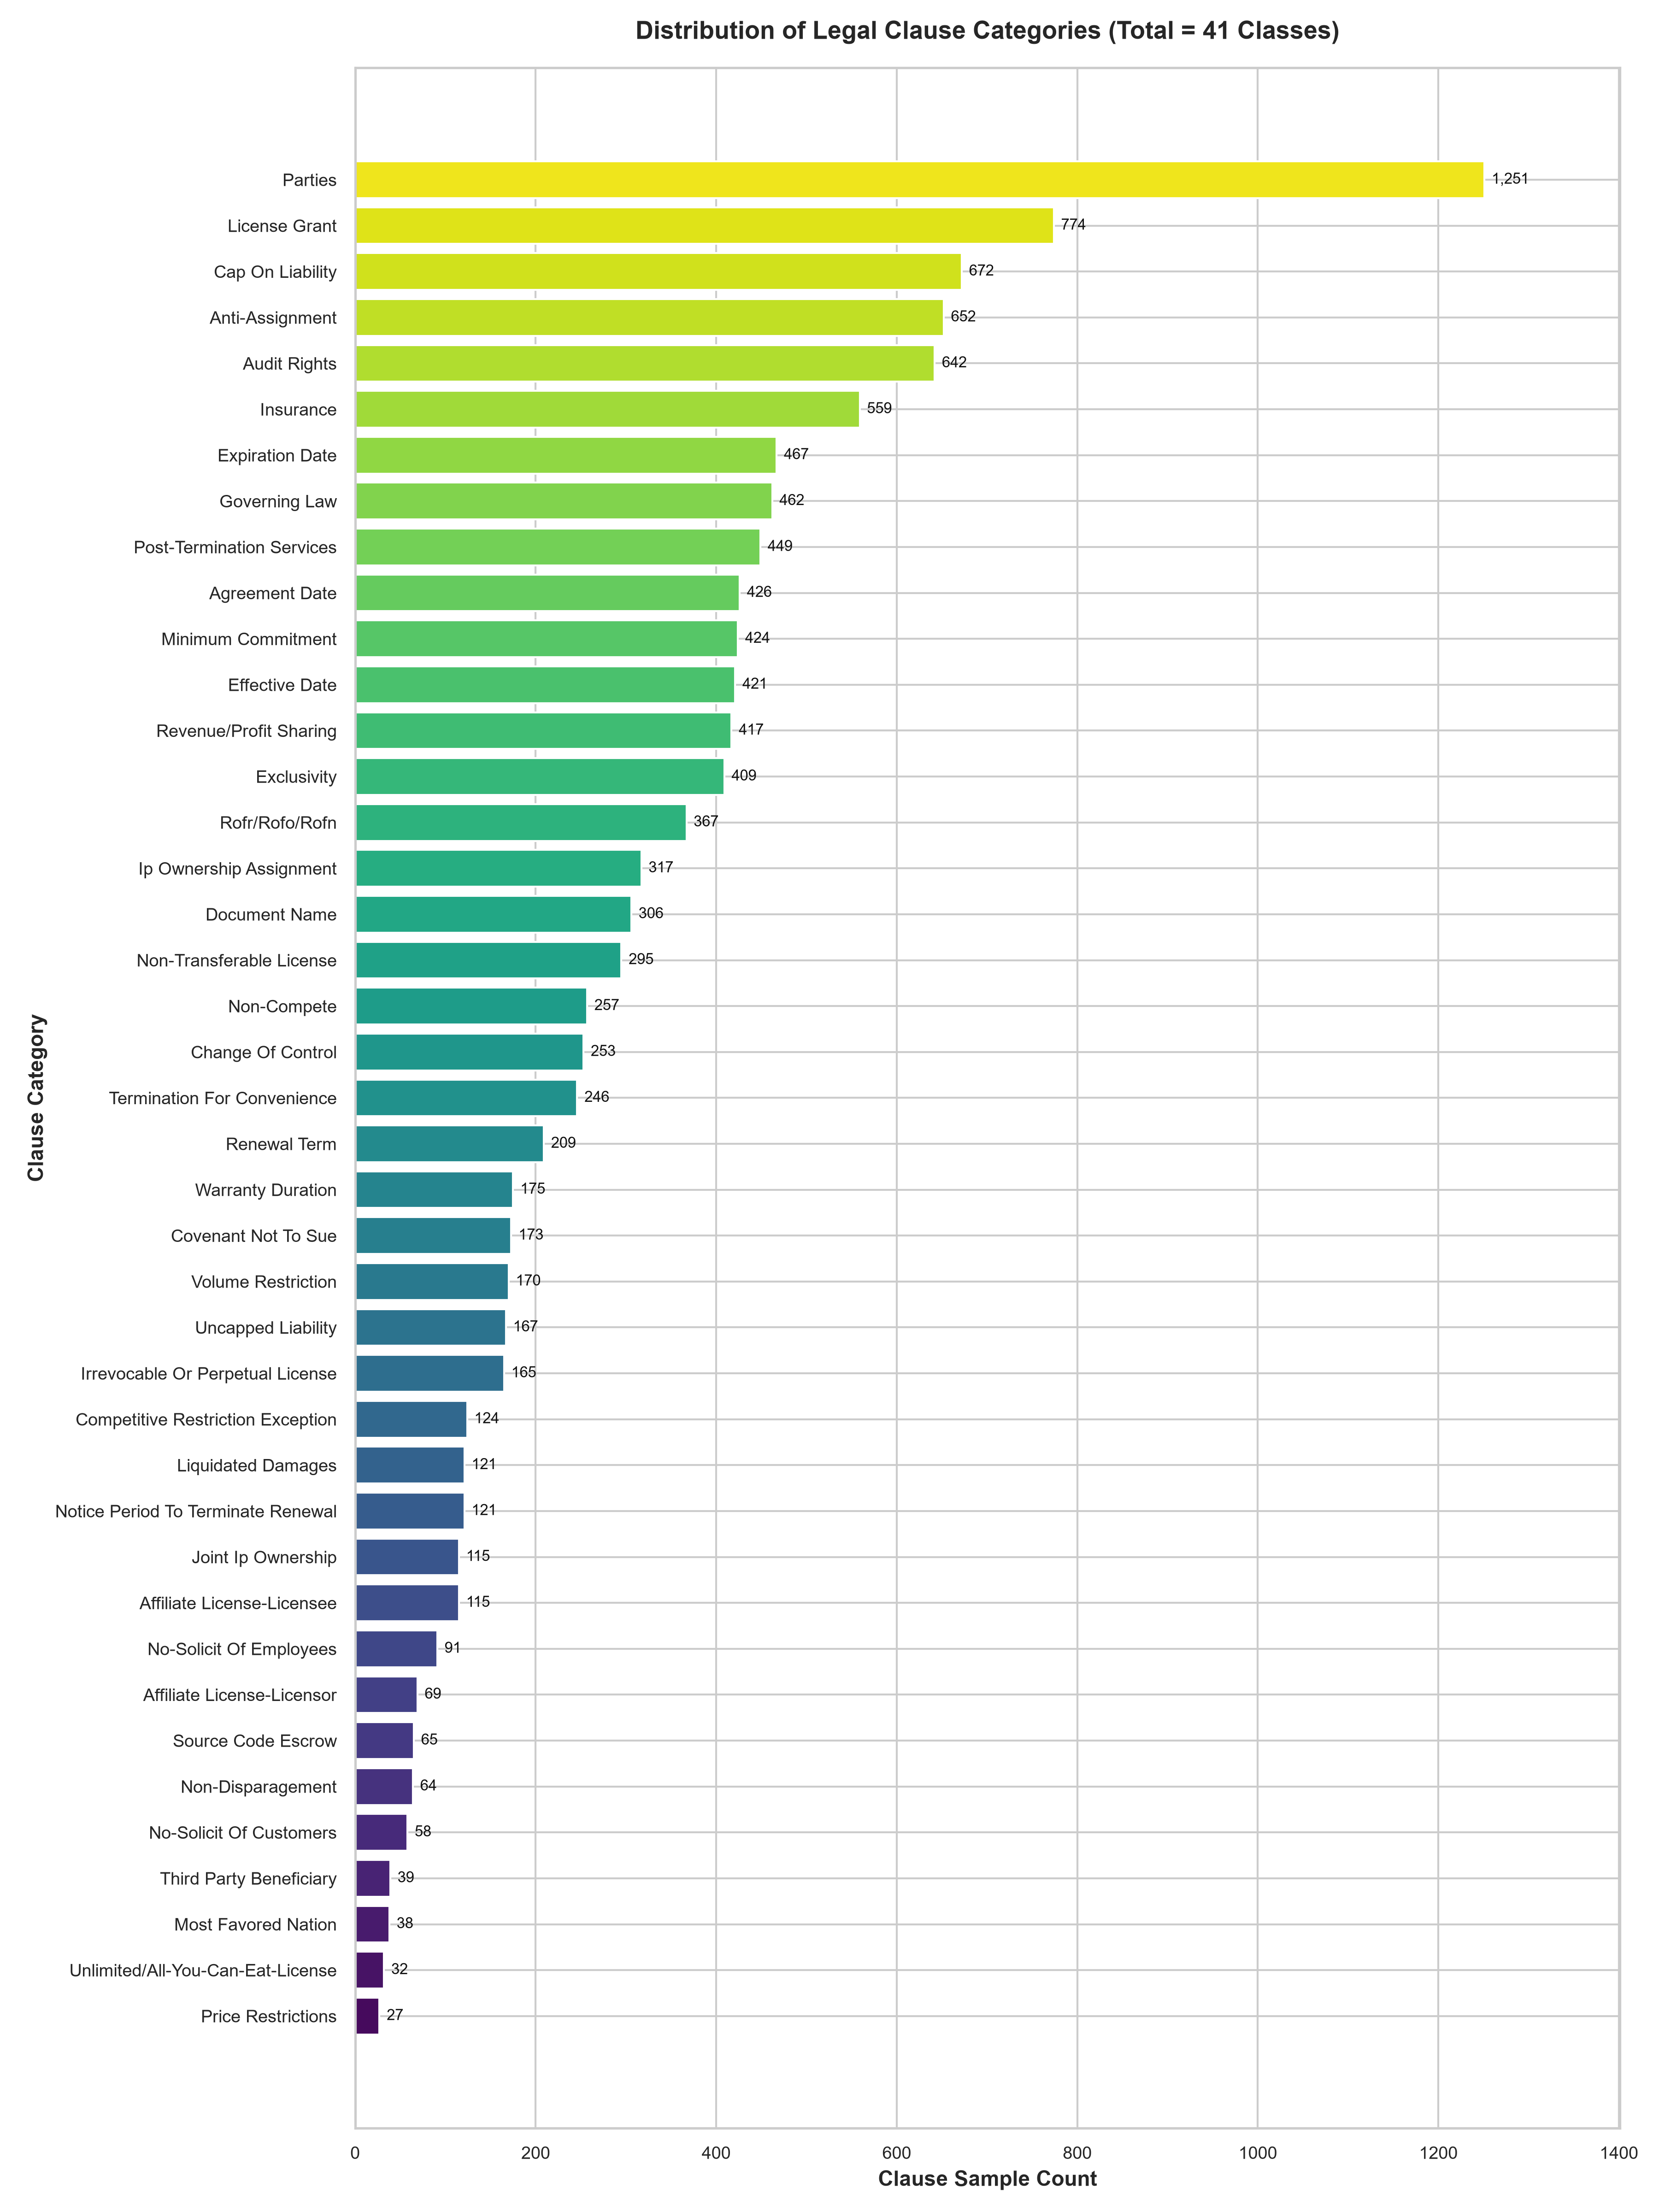
\includegraphics[width=0.92\textwidth]{figures/class_distribution.png}
\caption{Complete 41-category class distribution in the ClauseIQ dataset ($N = 12,204$)}
\label{fig:class_distribution}
\end{figure}

\subsection{Average Clause Word Count by Category}
Figure \ref{fig:avg_word_count} depicts the mean word count across categories. Factual metadata categories (\textit{Agreement Date}, \textit{Parties}) average under 6 words, whereas substantive covenants (\textit{Affiliate License-Licensor}, \textit{Irrevocable Or Perpetual License}) average between 80 and 95 words per clause.

\begin{figure}[h!]
\centering
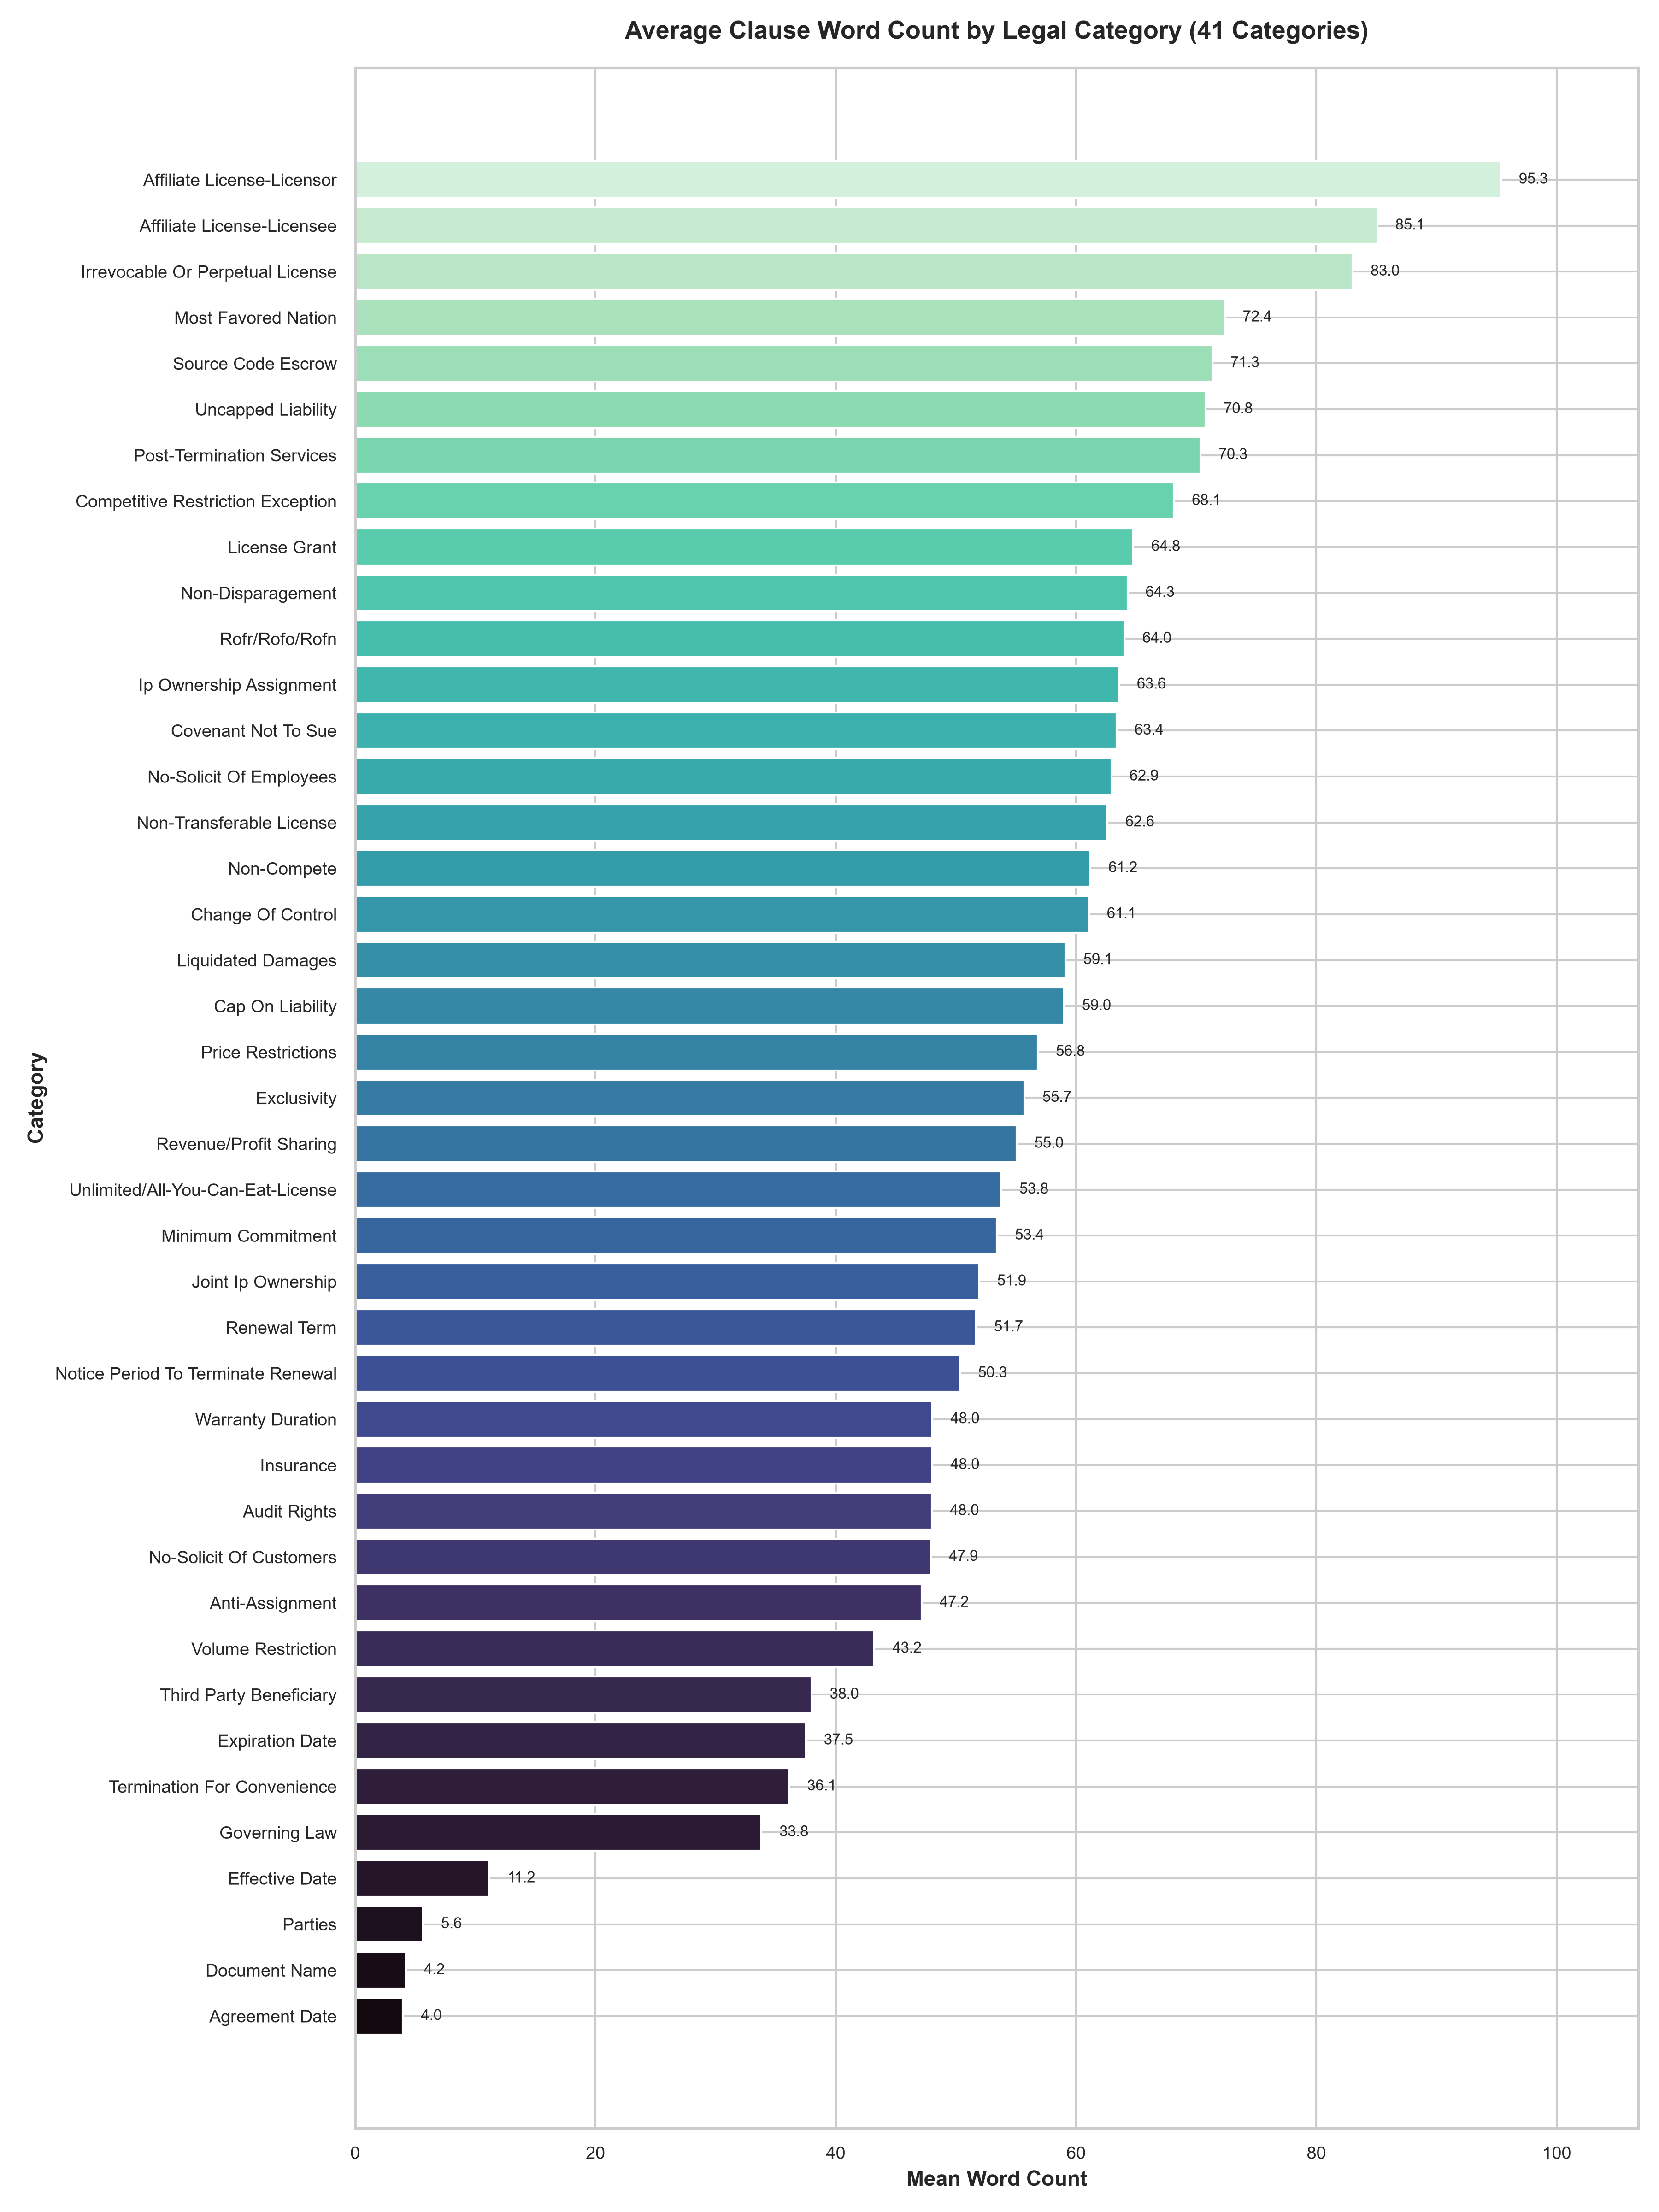
\includegraphics[width=0.92\textwidth]{figures/average_word_count_by_category.png}
\caption{Average clause word count across legal categories}
\label{fig:avg_word_count}
\end{figure}

\subsection{Word Count Distribution and Correlation Heatmap}
Figure \ref{fig:word_count_distribution} shows the right-skewed distribution of clause word counts across the dataset, with a sharp concentration between 15 and 50 words.

\begin{figure}[h!]
\centering
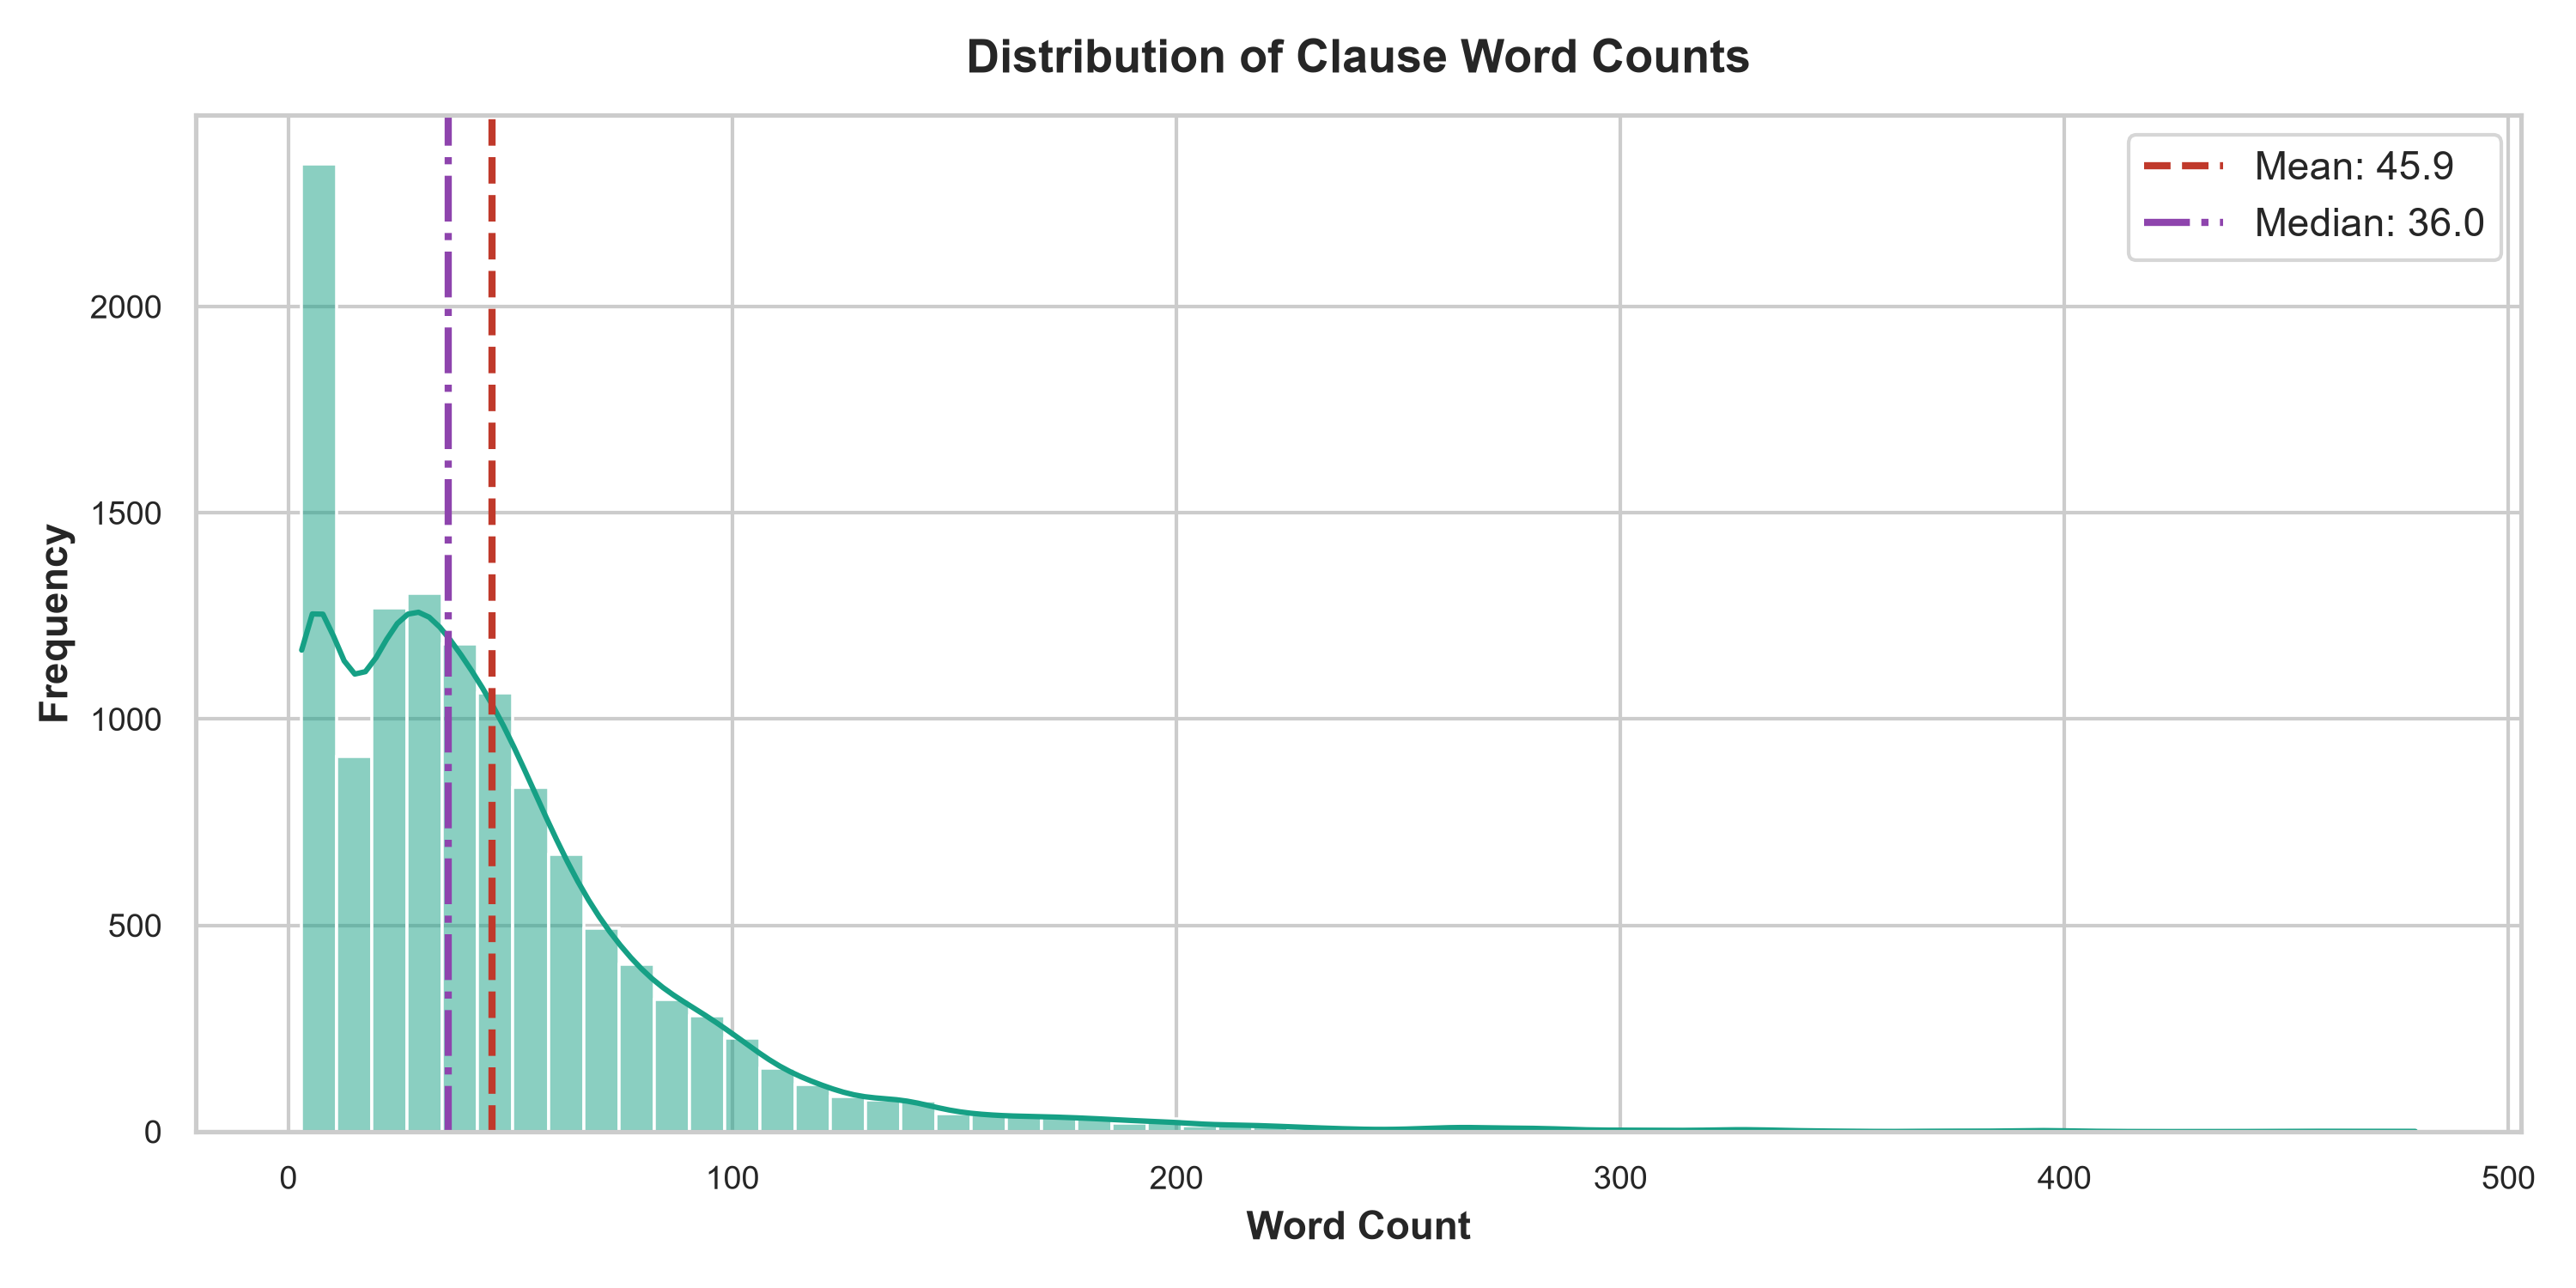
\includegraphics[width=0.85\textwidth]{figures/word_count_distribution.png}
\caption{Distribution of clause word counts}
\label{fig:word_count_distribution}
\end{figure}

Figure \ref{fig:correlation_heatmap} demonstrates the correlation matrix among length metrics; character length and word count display a near-perfect correlation of \textbf{0.9945}, confirming that character length provides no independent discriminatory signal beyond word count.

\begin{figure}[h!]
\centering
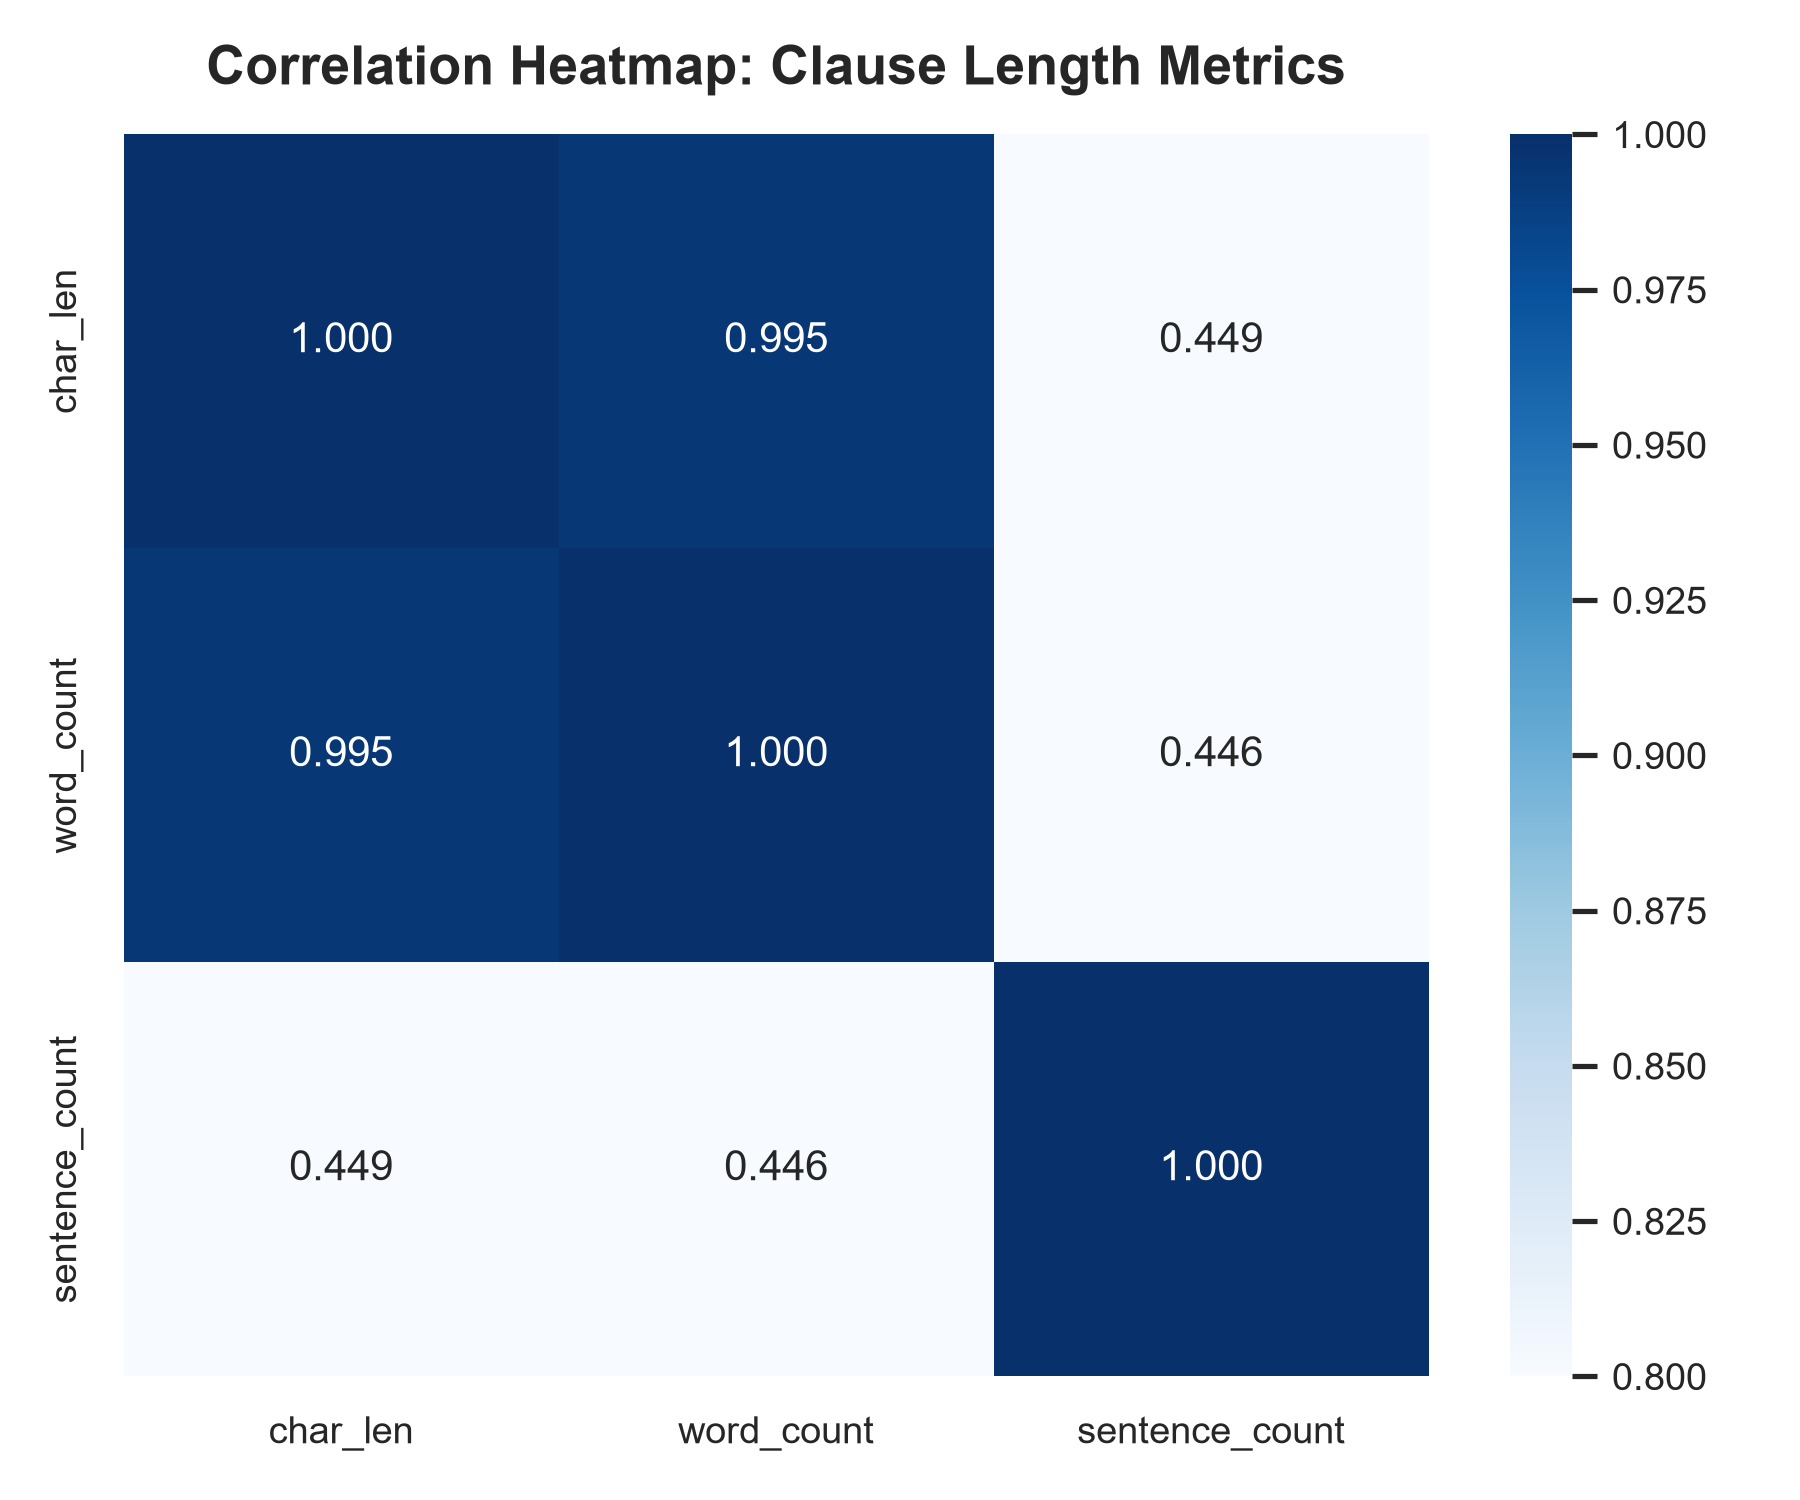
\includegraphics[width=0.85\textwidth]{figures/numerical_correlation.png}
\caption{Correlation matrix of text metrics}
\label{fig:correlation_heatmap}
\end{figure}

\subsection{Top Legal Bigrams}
Figure \ref{fig:top_bigrams} highlights the top 20 most frequent bigrams extracted from the corpus. Standard legal collocations—such as ``\textit{agreement shall}'', ``\textit{set forth}'', ``\textit{effective date}'', and ``\textit{prior written}''—dominate the feature space, justifying the use of bigram feature representations.

\begin{figure}[h!]
\centering
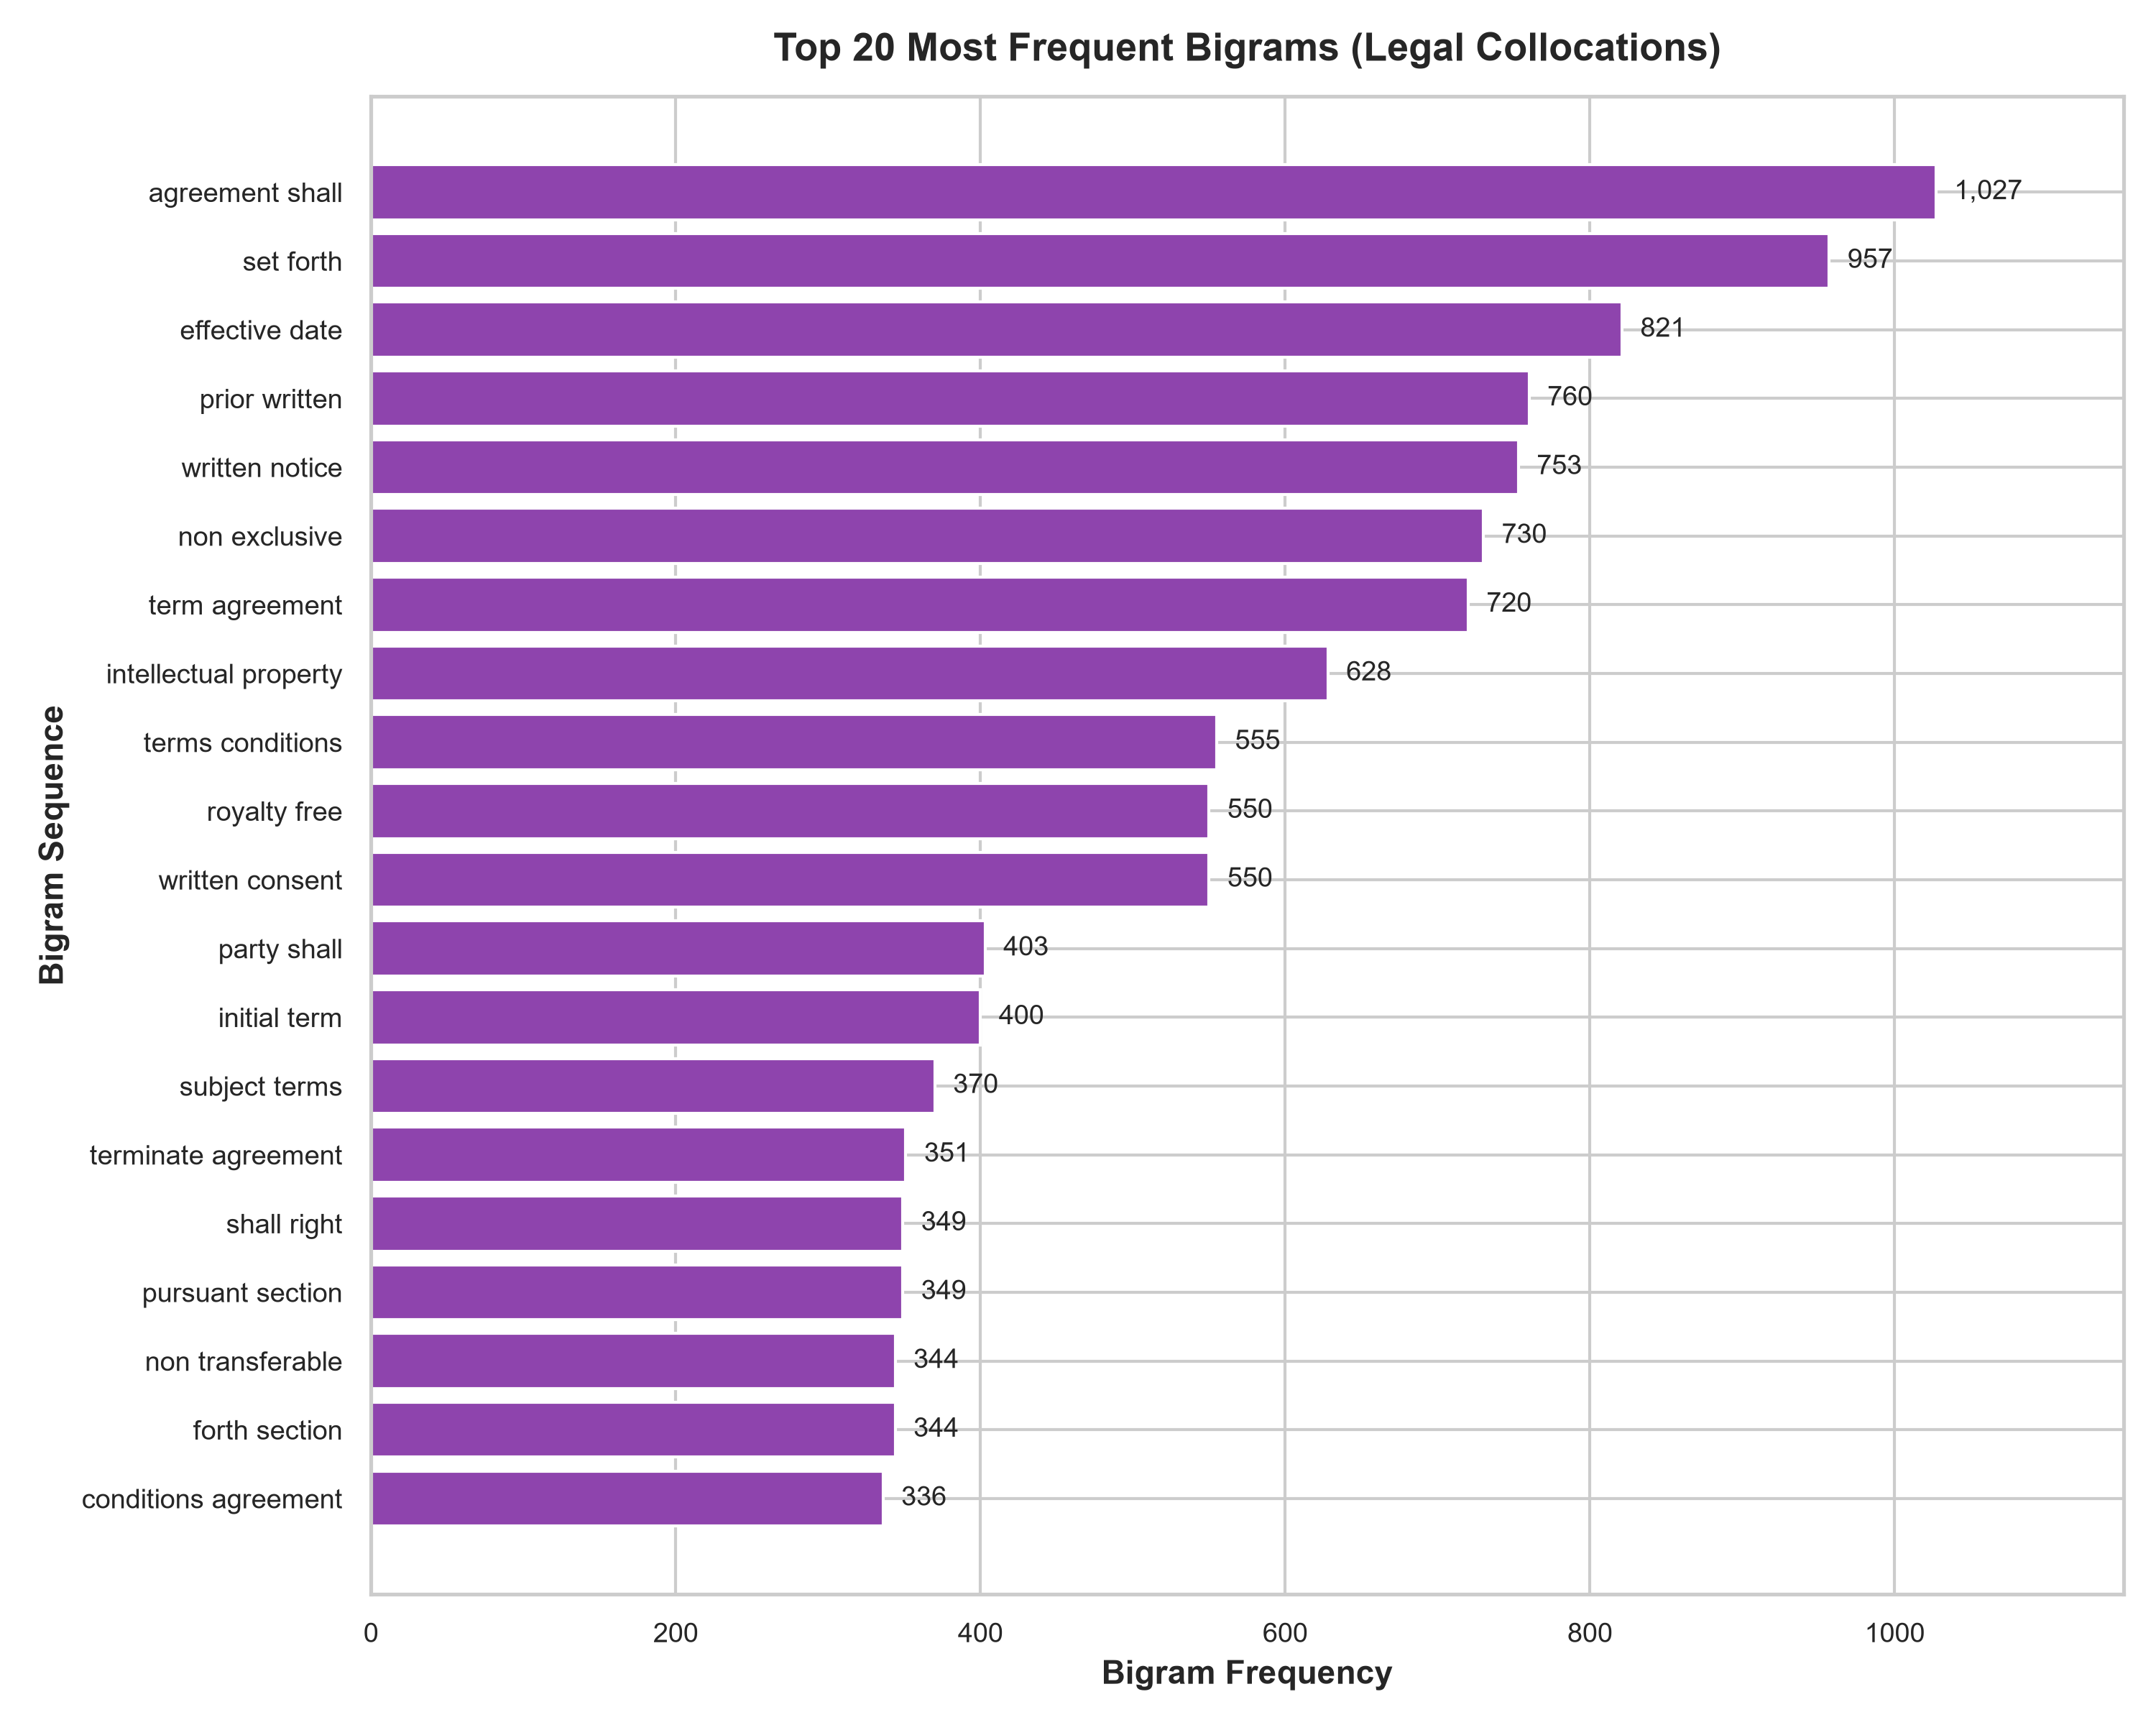
\includegraphics[width=0.85\textwidth]{figures/top_bigrams.png}
\caption{Top 20 most frequent bigrams in the ClauseIQ clause corpus}
\label{fig:top_bigrams}
\end{figure}

% ----------------------------------------------------------------------
% Section 3.4: Analysis of Architecture and(or) Algorithms
% ----------------------------------------------------------------------
\section{Analysis of Architecture and(or) Algorithms}
\label{sec:algorithms_analysis}

\subsection{Detailed Study Report of the Proposed Algorithm(s)}
\label{subsec:proposed_algorithms}
ClauseIQ unites a unified 10,000-dimensional TF-IDF vector space with four classical machine learning classifiers for automated clause categorization, and a vector similarity retrieval module for intelligent clause search.

\subsubsection*{1. TF-IDF Vectorization}
Term Frequency--Inverse Document Frequency converts unstructured text strings into normalized, sparse numerical vectors. 

The Term Frequency ($TF$) represents the normalized frequency of term $t$ in clause $d$:
\begin{equation}
    TF(t, d) = \frac{f_{t,d}}{\sum_{t' \in d} f_{t',d}}
\end{equation}
Under sublinear scaling, this is modified to $1 + \log(f_{t,d})$ for all $f_{t,d} > 0$.

The Inverse Document Frequency ($IDF$) measures the relative specificity of term $t$ across the entire corpus $D$ of $N$ clauses:
\begin{equation}
    IDF(t, D) = \log \left( \frac{1 + N}{1 + DF(t)} \right) + 1
\end{equation}
where $DF(t)$ is the number of clauses containing term $t$.

The composite TF-IDF score is computed as:
\begin{equation}
    TF\text{-}IDF(t, d, D) = TF(t, d) \times IDF(t, D)
\end{equation}
Each resulting vector is subsequently $L_2$-normalized:
\begin{equation}
    v_{\text{norm}} = \frac{v}{\|v\|_2}
\end{equation}

\subsubsection*{2. Multinomial Naive Bayes}
Multinomial Naive Bayes is a probabilistic classifier based on Bayes' theorem under the conditional independence assumption among features given the class label.

Given a feature vector $x = (t_1, t_2, \dots, t_n)$ representing a clause, the posterior probability of category $c$ is:
\begin{equation}
    P(c \mid x) \propto P(c) \prod_{i=1}^{n} P(t_i \mid c)^{f_i}
\end{equation}
where $P(c)$ is the prior probability of category $c$, and $P(t_i \mid c)$ is the probability of term $t_i$ occurring in category $c$.

To eliminate zero-probability errors for unseen terms, Lidstone/Laplace smoothing with parameter $\alpha$ is applied:
\begin{equation}
    P(t_i \mid c) = \frac{N_{ci} + \alpha}{N_c + \alpha |V|}
\end{equation}
where $N_{ci}$ is the sum of TF-IDF weights for term $t_i$ in class $c$, $N_c$ is the total sum across all vocabulary terms for class $c$, and $|V| = 10,000$.

\subsubsection*{3. Linear Support Vector Machine (Linear SVM)}
Support Vector Machines construct optimal separating hyperplanes that maximize the functional margin between classes in high-dimensional feature space. Linear SVM is exceptionally effective for sparse text classification where the feature dimensionality is large.

For multi-class classification across 41 categories, a One-vs-Rest (OvR) formulation is employed, training 41 binary linear classifiers. The primal optimization problem for each binary sub-problem is:
\begin{equation}
    \min_{w, b, \xi} \frac{1}{2} \|w\|^2 + C \sum_{i=1}^{m} \xi_i
\end{equation}
subject to the margin constraints:
\begin{equation}
    y_i (w^T x_i + b) \ge 1 - \xi_i, \quad \xi_i \ge 0, \quad \forall i \in \{1, \dots, m\}
\end{equation}
where $w$ is the normal weight vector, $b$ is the bias offset, $\xi_i$ are slack variables permitting soft-margin misclassifications, and $C$ is the regularization parameter governing the trade-off between margin width and training error.

\subsubsection*{4. Logistic Regression}
Logistic Regression is a discriminative linear model that predicts posterior class probabilities using the multinomial softmax function.

For a clause vector $x \in \mathbb{R}^{10000}$, the probability that it belongs to category $c \in \{1, \dots, 41\}$ is parameterized as:
\begin{equation}
    P(y = c \mid x) = \frac{\exp(w_c^T x + b_c)}{\sum_{j=1}^{41} \exp(w_j^T x + b_j)}
\end{equation}
where $w_c$ and $b_c$ denote the learned weights and intercept for class $c$.

The model parameters are optimized by minimizing the $L_2$-regularized cross-entropy loss across $m$ training samples:
\begin{equation}
    \mathcal{L}(W) = - \sum_{i=1}^{m} \sum_{c=1}^{41} \mathbb{I}(y_i = c) \log P(y_i = c \mid x_i) + \frac{1}{2C} \sum_{c=1}^{41} \|w_c\|_2^2
\end{equation}
Logistic Regression provides class probability estimates through its multinomial softmax formulation, enabling the generation of prediction confidence scores.

\subsubsection*{5. Random Forest Classifier}
Random Forest is an ensemble learning method that constructs a multitude of decision trees during training and outputs the majority voting class among individual trees.

To inject diversity and prevent overfitting on high-dimensional text vectors:
\begin{enumerate}
    \item \textbf{Bootstrap Aggregation (Bagging):} Each decision tree $T_b$ is trained on an independently drawn bootstrap sample of the training dataset.
    \item \textbf{Random Feature Subspaces:} At each internal split node, a random subset of features $\sqrt{|V|}$ is evaluated rather than the entire 10,000-dimensional feature space.
\end{enumerate}

Split quality is evaluated using the Gini Impurity metric:
\begin{equation}
    \text{Gini}(D) = 1 - \sum_{c=1}^{41} p_c^2
\end{equation}
where $p_c$ is the proportion of samples belonging to class $c$ in node $D$. The final ensemble prediction is obtained by majority vote:
\begin{equation}
    \hat{y} = \arg\max_c \sum_{b=1}^{B} \mathbb{I}(T_b(x) = c)
\end{equation}

\subsubsection*{6. Cosine Similarity (Intelligent Search)}
For the intelligent search engine, user queries and contract clauses are embedded into the same 10,000-dimensional TF-IDF vector space. The relevance of a candidate clause vector $B$ to a search query vector $A$ is quantified by calculating the cosine of the angle between them:
\begin{equation}
    \text{Similarity}(A, B) = \cos(\theta) = \frac{A \cdot B}{\|A\|_2 \|B\|_2} = \frac{\sum_{i=1}^{10000} A_i B_i}{\sqrt{\sum_{i=1}^{10000} A_i^2} \sqrt{\sum_{i=1}^{10000} B_i^2}}
\end{equation}

Because both query and clause vectors are $L_2$-normalized during vectorization ($\|A\|_2 = \|B\|_2 = 1$), the cosine similarity simplifies to the efficient sparse dot product:
\begin{equation}
    \text{Similarity}(A, B) = A \cdot B = \sum_{i=1}^{10000} A_i B_i
\end{equation}
Cosine similarity is strictly scale-invariant, preventing longer clauses from receiving artificially elevated scores purely due to document length.

\subsubsection*{7. Performance Evaluation Metrics}
To assess classification performance objectively, standard evaluation metrics are computed on the held-out test split:
\begin{itemize}
    \item \textbf{Precision ($P_c$):} $\frac{TP_c}{TP_c + FP_c}$ (Proportion of predicted class $c$ clauses that are correct).
    \item \textbf{Recall ($R_c$):} $\frac{TP_c}{TP_c + FN_c}$ (Proportion of actual class $c$ clauses correctly identified).
    \item \textbf{Accuracy:} $\frac{\sum_{c=1}^{41} TP_c}{N_{\text{total}}}$ (Overall percentage of correct predictions across all samples).
    \item \textbf{Class F1-Score ($F1_c$):} $2 \times \frac{P_c \times R_c}{P_c + R_c}$ (Harmonic mean of precision and recall for class $c$).
    \item \textbf{Macro-F1:} $\frac{1}{41} \sum_{c=1}^{41} F1_c$ (\textbf{Primary selection metric}; weights all 41 categories equally).
    \item \textbf{Weighted-F1:} $\sum_{c=1}^{41} \left( \frac{N_c}{N_{\text{total}}} \right) F1_c$ (Weights F1 by category sample proportion).
\end{itemize}

\noindent\textbf{Critical Conceptual Distinction:} Macro-F1 is an aggregate classification performance metric calculated over an evaluation dataset. It is not a probability, confidence score, or indicator of the likelihood of an individual prediction. Logistic Regression provides class probability estimates through its multinomial softmax formulation. These probability estimates are distinct from the Macro-F1 evaluation metric.

% ----------------------------------------------------------------------
% Section 3.5: Project Pipeline
% ----------------------------------------------------------------------
\section{Project Pipeline}
\label{sec:project_pipeline}
Figure \ref{fig:project_pipeline} illustrates the multi-stage operational pipeline of ClauseIQ.

\begin{figure}[h!]
\centering
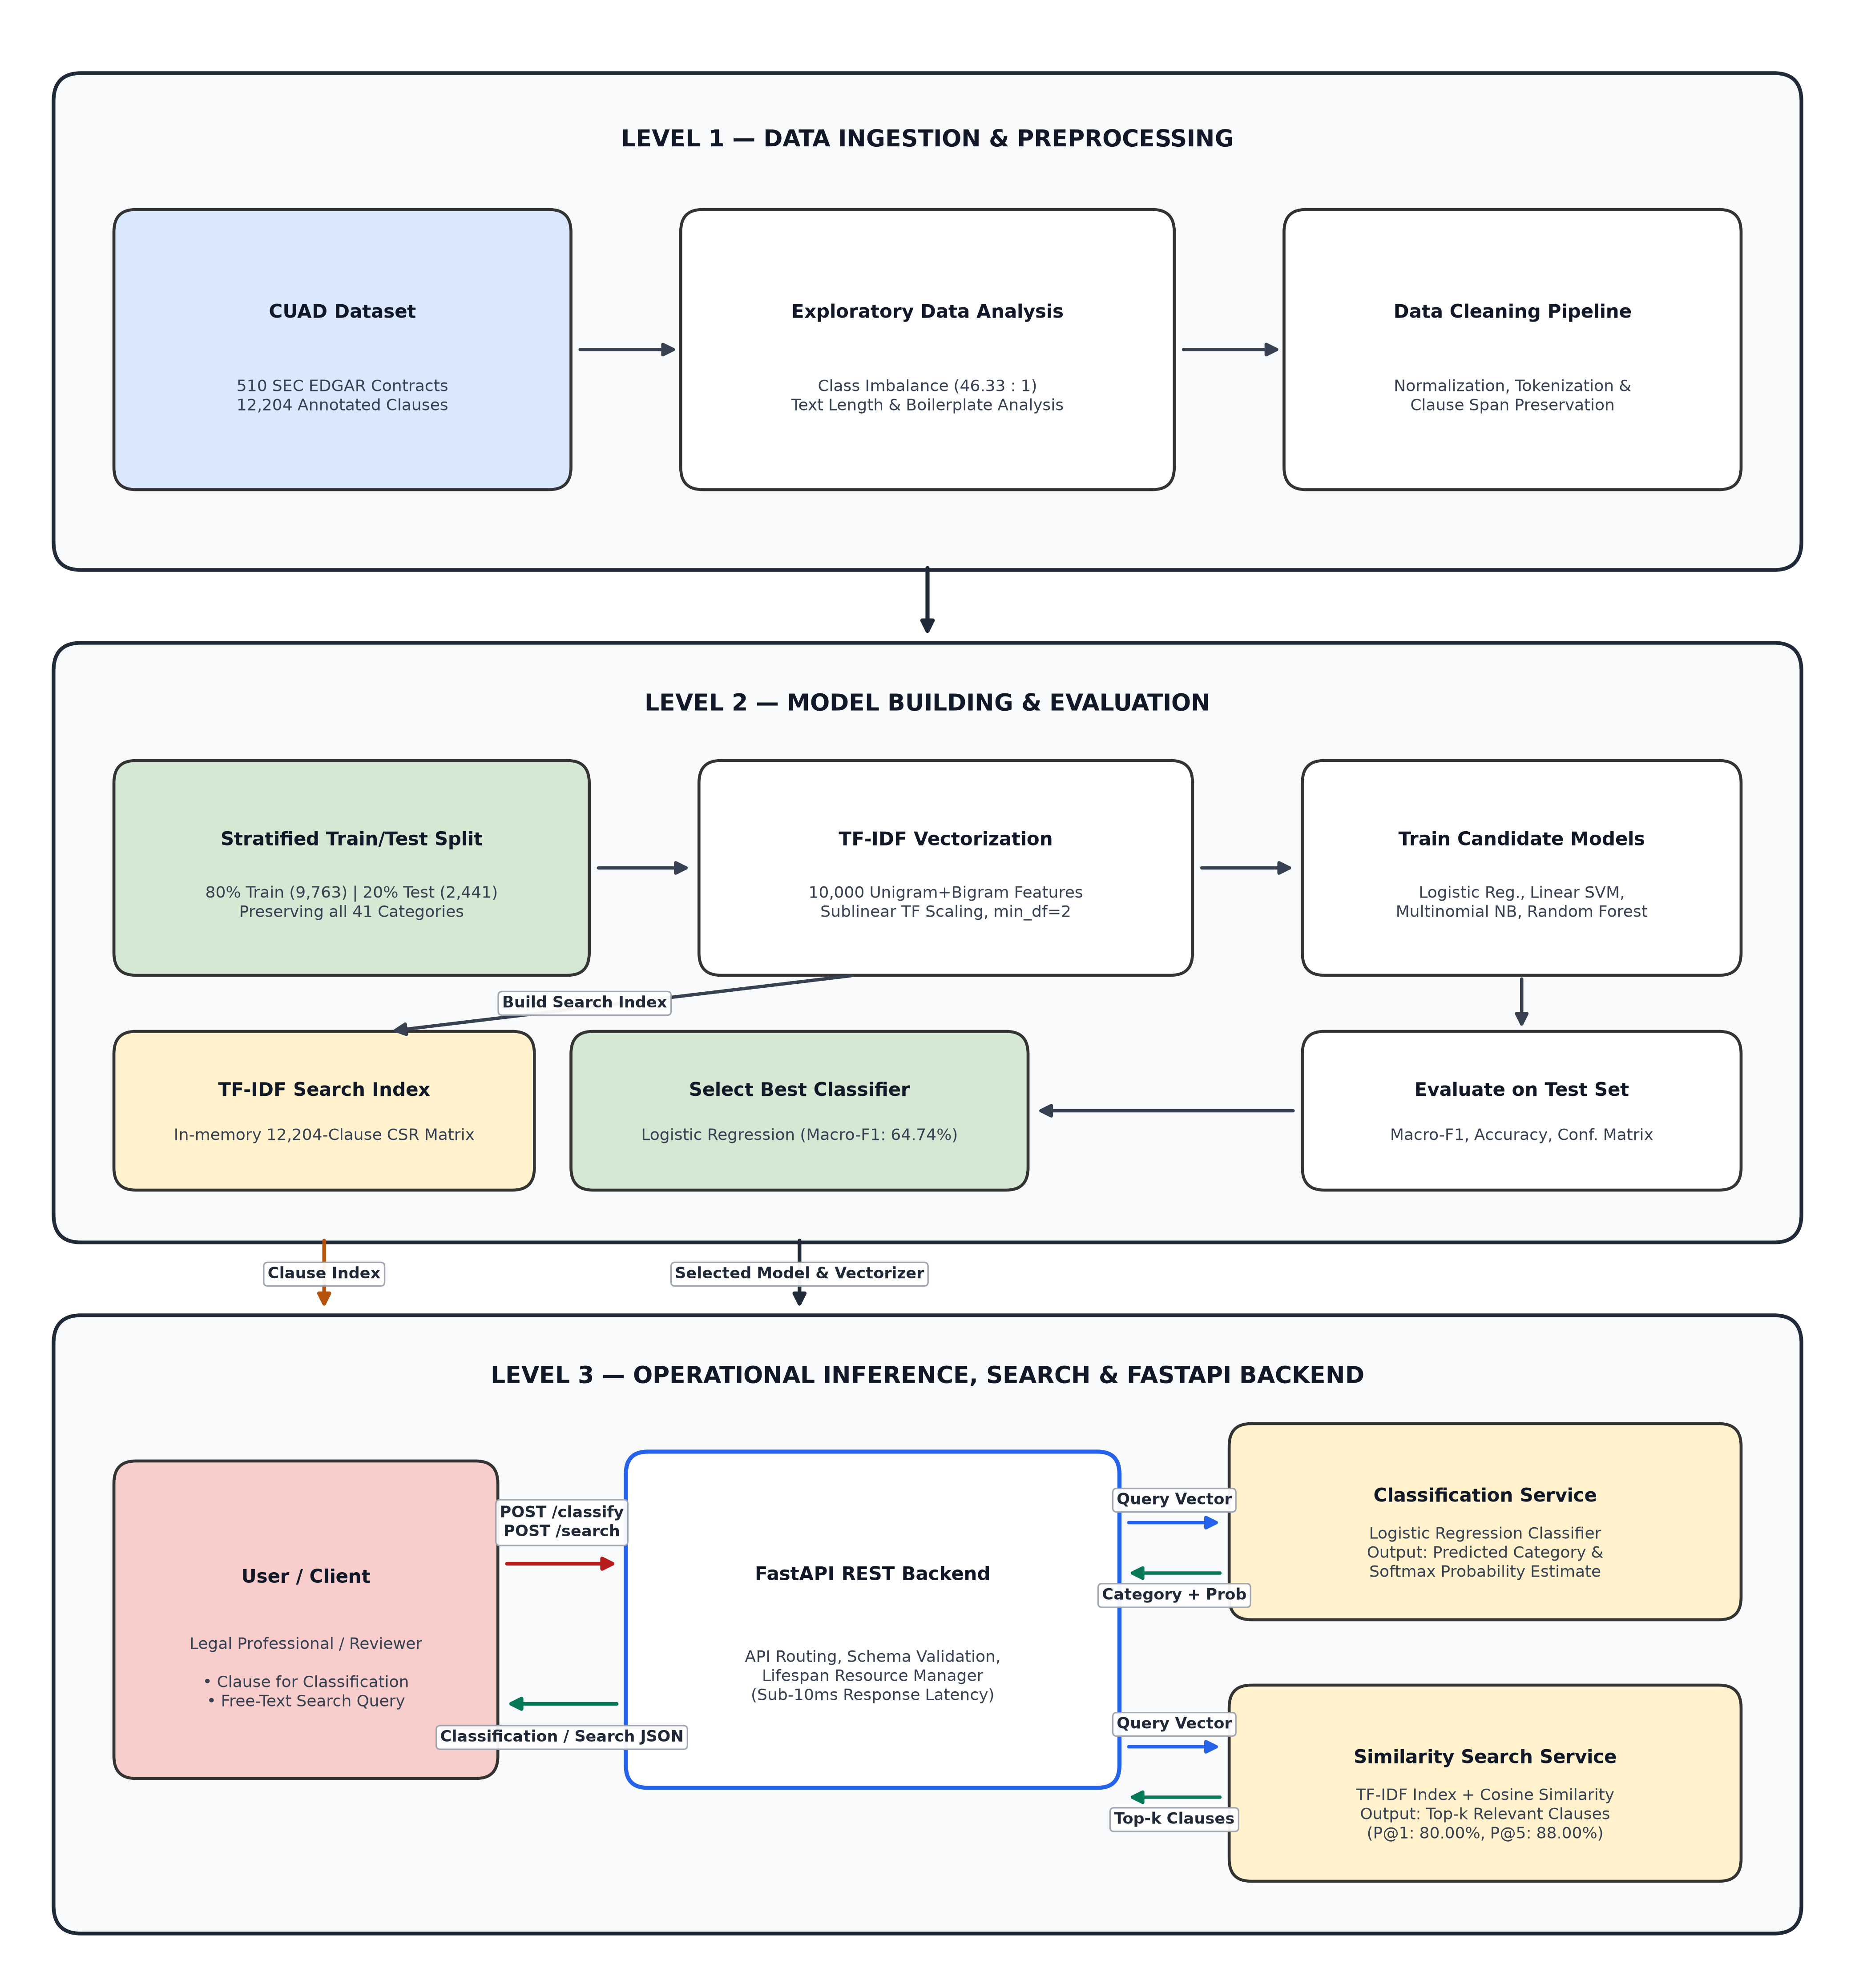
\includegraphics[width=0.85\textwidth]{figures/project_pipeline.png}
\caption{End-to-end ClauseIQ system pipeline architecture}
\label{fig:project_pipeline}
\end{figure}

The pipeline executes through structured operational stages:
\begin{enumerate}
    \item \textbf{Data Ingestion \& Flattening:} Raw CUAD contract JSON annotations are ingested and flattened into a structured tabular schema with 12,204 rows and 41 classes.
    \item \textbf{Data Cleaning \& Stratification:} Normalization, tokenization, and stratified 80/20 train/test splitting ($N_{\text{train}} = 9,763$, $N_{\text{test}} = 2,441$).
    \item \textbf{Feature Extraction:} Fitting of the 10,000-feature unigram+bigram TF-IDF vectorizer with sublinear scaling on the training split.
    \item \textbf{Model Training \& Tuning:} Training and cross-validated tuning of four classical machine learning classifiers.
    \item \textbf{Evaluation \& Selection:} Comprehensive multi-metric benchmark on the held-out test split to identify the optimal production classifier based on Macro-F1.
    \item \textbf{Search Indexing:} Construction of an in-memory sparse CSR vector index over all 12,204 clauses for sub-10ms Cosine Similarity retrieval.
    \item \textbf{API Serving:} Packaging model artifacts and the search engine inside FastAPI REST endpoints.
\end{enumerate}

% ----------------------------------------------------------------------
% Section 3.6: Feasibility Analysis
% ----------------------------------------------------------------------
\section{Feasibility Analysis}
\label{sec:feasibility_analysis}
A comprehensive feasibility assessment was conducted across technical, economic, and operational dimensions.

\subsubsection*{Technical Feasibility}
\begin{itemize}
    \item \textbf{Software Maturity:} The entire machine learning and search pipeline is constructed using industry-standard, battle-tested Python libraries (\texttt{scikit-learn}, \texttt{pandas}, \texttt{numpy}, \texttt{FastAPI}). No specialized or experimental frameworks are required.
    \item \textbf{Hardware Constraints:} Classical machine learning algorithms require modest computational resources. Model training across 12,204 samples executes in under three minutes on a standard quad-core CPU without GPU acceleration.
    \item \textbf{Algorithmic Reliability:} Deterministic mathematical operations (TF-IDF vector dot products) ensure reproducible, verifiable retrieval without stochastic variation or hallucination risks.
\end{itemize}

\subsubsection*{Economic Feasibility}
The system incurs zero software licensing costs. All utilized components—Python, scikit-learn, FastAPI, and the CUAD dataset (licensed under Creative Commons Attribution 4.0 International)—are entirely open-source and free for academic and commercial use. Because the system runs efficiently on existing commodity laptops and low-cost server instances, hardware acquisition and operational hosting costs remain virtually zero.

\subsubsection*{Operational Feasibility}
From an operational perspective, the system delivers immediate utility to legal workflows. Reviewers are not required to understand vector spaces or machine learning mathematics. Through standardized RESTful API endpoints, users submit raw clause text to receive immediate category classifications with confidence scores, or submit search queries to obtain relevance-ranked clause matches in milliseconds.

% ----------------------------------------------------------------------
% Section 3.7: System Environment
% ----------------------------------------------------------------------
\section{System Environment}
\label{sec:system_environment}

\subsection{Software Environment}
\begin{itemize}
    \item \textbf{Operating System:} Microsoft Windows 11 / Linux (Ubuntu 22.04 LTS compatible).
    \item \textbf{Programming Language:} Python 3.10+ (Current runtime: Python 3.14.6 64-bit).
    \item \textbf{Core ML Libraries:} \texttt{scikit-learn} (v1.9.0), \texttt{scipy} (v1.18.0), \texttt{numpy} (v2.5.2).
    \item \textbf{Data Processing:} \texttt{pandas} (v3.0.5), \texttt{regex}, \texttt{joblib} (v1.5.3).
    \item \textbf{Web Framework:} \texttt{FastAPI} (v0.141.1), \texttt{uvicorn} (v0.54.0), \texttt{pydantic} (v2.13.5).
    \item \textbf{Automated Testing:} \texttt{pytest} (v9.1.1).
    \item \textbf{Visualization:} \texttt{matplotlib} (v3.11.1), \texttt{seaborn} (v0.13.2).
\end{itemize}

\subsection{Hardware Environment}
\begin{itemize}
    \item \textbf{Processor:} Multi-core Intel Core i5/i7 (8th Gen or newer) or AMD Ryzen 5/7.
    \item \textbf{Random Access Memory (RAM):} 8.0\,GB minimum (16.0\,GB recommended).
    \item \textbf{Storage:} 10.0\,GB available Solid State Drive (SSD) storage.
    \item \textbf{GPU:} None required (all processing executes on CPU).
\end{itemize}

\chapter{SYSTEM DESIGN}
\label{ch:system_design}

This chapter details the system design, dataset splitting strategy, feature extraction pipeline, model training workflows, and hyperparameter optimization methodologies for the four classical machine learning classifiers evaluated in ClauseIQ.

% ----------------------------------------------------------------------
% Section 4.1: Model(s) Building
% ----------------------------------------------------------------------
\section{Model(s) Building}
\label{sec:model_building}

\subsection{Implementation Code}
\label{subsec:implementation_code}
The model-building subsystem is engineered to ensure reproducible, modular execution without data leakage. The implementation is organized into four core functional modules:
\begin{enumerate}
    \item \textbf{Text Normalization and Ingestion Module (\texttt{src/clean\_dataset.py}):} Loads the cleaned 12,204-clause corpus from \texttt{data/clauseiq\_dataset\_clean.csv}, verifying column schemas and label encodings.
    \item \textbf{Stratified Splitting Module (\texttt{src/clean\_dataset.py}):} Generates reproducible train and test subsets while strictly preserving per-class label proportions across all 41 categories.
    \item \textbf{TF-IDF Feature Extraction Module (\texttt{src/feature\_extraction.py}):} Fits the vocabulary exclusively on training text samples and applies sparse transformations across both subsets.
    \item \textbf{Classifier Training and Optimization Module (\texttt{src/train\_baseline.py}, \texttt{src/train\_svm.py}, \texttt{src/train\_nb.py}, \texttt{src/train\_random\_forest.py}):} Trains and tunes the four candidate machine learning algorithms using cross-validation on the training set, serializing the final estimators and vectorizers for model evaluation and API serving.
\end{enumerate}

\subsection{Model Planning (Training/Testing split of the dataset)}
\label{subsec:model_planning}
In legal natural language processing, partitioning the dataset must be performed with extreme care. Because the dataset exhibits a severe 46.33:1 class imbalance across 41 categories, an unstratified random split would result in extreme undersampling or complete absence of rare categories (such as \textit{Price Restrictions} with 27 total instances or \textit{Third Party Beneficiary} with 39 instances) from the test evaluation set.

To guarantee rigorous statistical representation, a \textbf{stratified 80/20 train/test split} was executed using \texttt{train\_test\_split} with \texttt{random\_state=42} and stratification governed by the target label array.

The verified sample counts of the split are:
\begin{itemize}
    \item \textbf{Total Corpus Records:} 12,204 samples
    \item \textbf{Training Split ($N_{\text{train}}$):} \textbf{9,763 samples} (80.0\%)
    \item \textbf{Testing Split ($N_{\text{test}}$):} \textbf{2,441 samples} (20.0\%)
    \item \textbf{Number of Classes Represented:} \textbf{41 classes} in both training and testing sets
    \item \textbf{Missing Classes in Either Split:} \textbf{0} (full class preservation verified)
\end{itemize}

The split artifacts were serialized directly to \texttt{models/train\_test\_split.pkl}, guaranteeing that all four machine learning models are evaluated on the \textbf{exact same held-out test instances}.

\subsubsection*{Feature Representation and Vectorization}
Feature extraction is performed by fitting \texttt{TfidfVectorizer} exclusively on the 9,763 training samples to prevent data leakage from the test split. The parameters are:
\begin{itemize}
    \item \textbf{Max Features:} \textbf{10,000 features}
    \item \textbf{N-gram Range:} $(1, 2)$ (capturing unigram vocabulary and bigram collocations)
    \item \textbf{Sublinear Term Frequency:} Enabled ($\text{sublinear\_tf} = \text{True}$)
    \item \textbf{Minimum Document Frequency:} $\text{min\_df} = 2$
\end{itemize}

Applying this vectorizer produces a sparse Compressed Sparse Row (CSR) matrix of shape $(9763, 10000)$ for training and $(2441, 10000)$ for testing.

\subsection{Training}
\label{subsec:training}
Four classical machine learning algorithms were trained and evaluated:
\begin{enumerate}
    \item Multinomial Naive Bayes
    \item Random Forest Classifier
    \item Linear Support Vector Machine (Linear SVM)
    \item Multinomial Logistic Regression
\end{enumerate}

To ensure optimal performance under class imbalance, hyperparameter tuning was conducted using Stratified K-Fold Cross-Validation, scoring candidates explicitly on \textbf{Macro-F1} (\texttt{scoring='f1\_macro'}).

\subsubsection*{1. Multinomial Naive Bayes Optimization (\texttt{src/train\_nb.py})}
Multinomial Naive Bayes does not natively support class weighting. Consequently, systematic tuning of the additive smoothing parameter $\alpha$ is required to prevent majority classes from overwhelming posterior probabilities.
\begin{itemize}
    \item \textbf{Tuning Strategy:} \texttt{GridSearchCV} with 5-fold Stratified Cross-Validation.
    \item \textbf{Candidate Search Space:} $\alpha \in \{0.001, 0.01, 0.05, 0.1, 0.2, 0.5, 1.0, 2.0\}$ (8 candidates).
    \item \textbf{Optimization Objective:} \texttt{f1\_macro}.
    \item \textbf{Optimal Parameter:} $\alpha = \mathbf{0.01}$.
    \item \textbf{Cross-Validation Performance:} Best 5-fold CV Macro-F1 = \textbf{0.5905}.
\end{itemize}

\subsubsection*{2. Random Forest Classifier Optimization (\texttt{src/train\_random\_forest.py})}
Due to the computational complexity of training ensembles across 10,000 sparse dimensions, hyperparameter optimization was conducted using randomized parameter search:
\begin{itemize}
    \item \textbf{Tuning Strategy:} \texttt{RandomizedSearchCV} with 3-fold Stratified Cross-Validation.
    \item \textbf{Iterations Evaluated:} 8 parameter configurations.
    \item \textbf{Parameter Search Grid:}
    \begin{itemize}
        \item \texttt{n\_estimators}: $[100, 150, 200]$
        \item \texttt{max\_depth}: $[30, 50, \text{None}]$
        \item \texttt{min\_samples\_split}: $[2, 5, 10]$
        \item \texttt{class\_weight}: $[\text{'balanced'}, \text{'balanced\_subsample'}]$
    \end{itemize}
    \item \textbf{Optimal Parameters Identified:}
    \begin{itemize}
        \item $\text{n\_estimators} = \mathbf{200}$
        \item $\text{min\_samples\_split} = \mathbf{10}$
        \item $\text{max\_depth} = \mathbf{50}$
        \item $\text{class\_weight} = \mathbf{\text{'balanced'}}$
    \end{itemize}
    \item \textbf{Cross-Validation Performance:} Best 3-fold CV Macro-F1 = \textbf{0.5776}.
\end{itemize}

\subsubsection*{3. Linear Support Vector Machine (\texttt{src/train\_svm.py})}
Linear SVM was trained using the One-vs-Rest (OvR) multiclass scheme with balanced class weighting:
\begin{itemize}
    \item \textbf{Kernel:} Linear.
    \item \textbf{Regularization Parameter:} $C = 0.1$.
    \item \textbf{Loss Function:} Squared hinge loss.
    \item \textbf{Class Weighting:} \texttt{class\_weight='balanced'}, scaling the penalty inversely proportional to category frequency.
\end{itemize}

\subsubsection*{4. Logistic Regression (\texttt{src/train\_baseline.py})}
Multinomial Logistic Regression was parameterized as follows:
\begin{itemize}
    \item \textbf{Formulation:} Multinomial cross-entropy (softmax loss).
    \item \textbf{Regularization:} $L_2$ penalty with inverse regularization strength $C = 1.0$.
    \item \textbf{Optimization Solver:} L-BFGS (Limited-memory Broyden--Fletcher--Goldfarb--Shanno).
    \item \textbf{Maximum Iterations:} 1,000 (ensuring complete convergence).
    \item \textbf{Class Weighting:} \texttt{class\_weight='balanced'}.
\end{itemize}

\subsection{Testing}
\label{subsec:testing}
Once trained and tuned on the training split, all four estimators were evaluated on the \textbf{exact same held-out test dataset} ($N = 2,441$). Test samples were transformed using the persisted vectorizer and passed through each model's prediction pipeline.

Classification performance was comprehensively assessed by computing scikit-learn's classification report across all 41 categories, generating full $41 \times 41$ confusion matrices, and logging accuracy, precision, recall, macro-averaged metrics, and weighted-averaged metrics. The empirical findings are detailed in Chapter \ref{ch:results_and_discussion}.

\chapter{RESULTS AND DISCUSSION}
\label{ch:results_and_discussion}

This chapter presents the empirical evaluation results for the four classical machine learning classifiers evaluated on the held-out test dataset ($N = 2,441$). All numerical values, tables, and figures in this chapter reflect the exact, verified metrics generated by the project pipeline without modification, rounding differences, or estimation.

% ----------------------------------------------------------------------
% Section 5.1: Comparison of Models
% ----------------------------------------------------------------------
\section{Comparison of Models}
\label{sec:comparison_of_models}

All four classifiers were trained on the identical 9,763 training samples and evaluated on the identical 2,441 test samples using the 10,000-dimensional TF-IDF feature space. Table \ref{tab:model_comparison} presents the comprehensive comparative benchmark across all primary and secondary evaluation metrics.

\begin{table}[h!]
\centering
\small
\begin{tabular}{lcccccc}
\toprule
\textbf{Model} & \textbf{Accuracy} & \textbf{Macro Prec} & \textbf{Macro Rec} & \textbf{Macro F1} & \textbf{Wtd Prec} & \textbf{Wtd F1} \\
\midrule
\textbf{Logistic Regression}  & 71.90\% & \textbf{64.81\%} & 66.22\% & \textbf{64.74\%} & \textbf{73.54\%} & 71.96\% \\
\textbf{Linear SVM}           & \textbf{72.63\%} & 63.23\% & \textbf{66.65\%} & 64.18\% & 73.31\% & \textbf{72.26\%} \\
\textbf{Multinomial NB}       & 69.27\% & 60.24\% & 58.67\% & 58.53\% & 69.96\% & 69.03\% \\
\textbf{Random Forest}        & 65.46\% & 55.27\% & 59.04\% & 56.34\% & 65.77\% & 64.96\% \\
\bottomrule
\end{tabular}
\caption{Comprehensive performance comparison across all 4 machine learning models ($N_{\text{test}} = 2,441$)}
\label{tab:model_comparison}
\end{table}

Figure \ref{fig:model_comparison_chart} visualizes the performance comparison across Accuracy, Macro-F1, and Weighted-F1 scores.

\begin{figure}[h!]
\centering
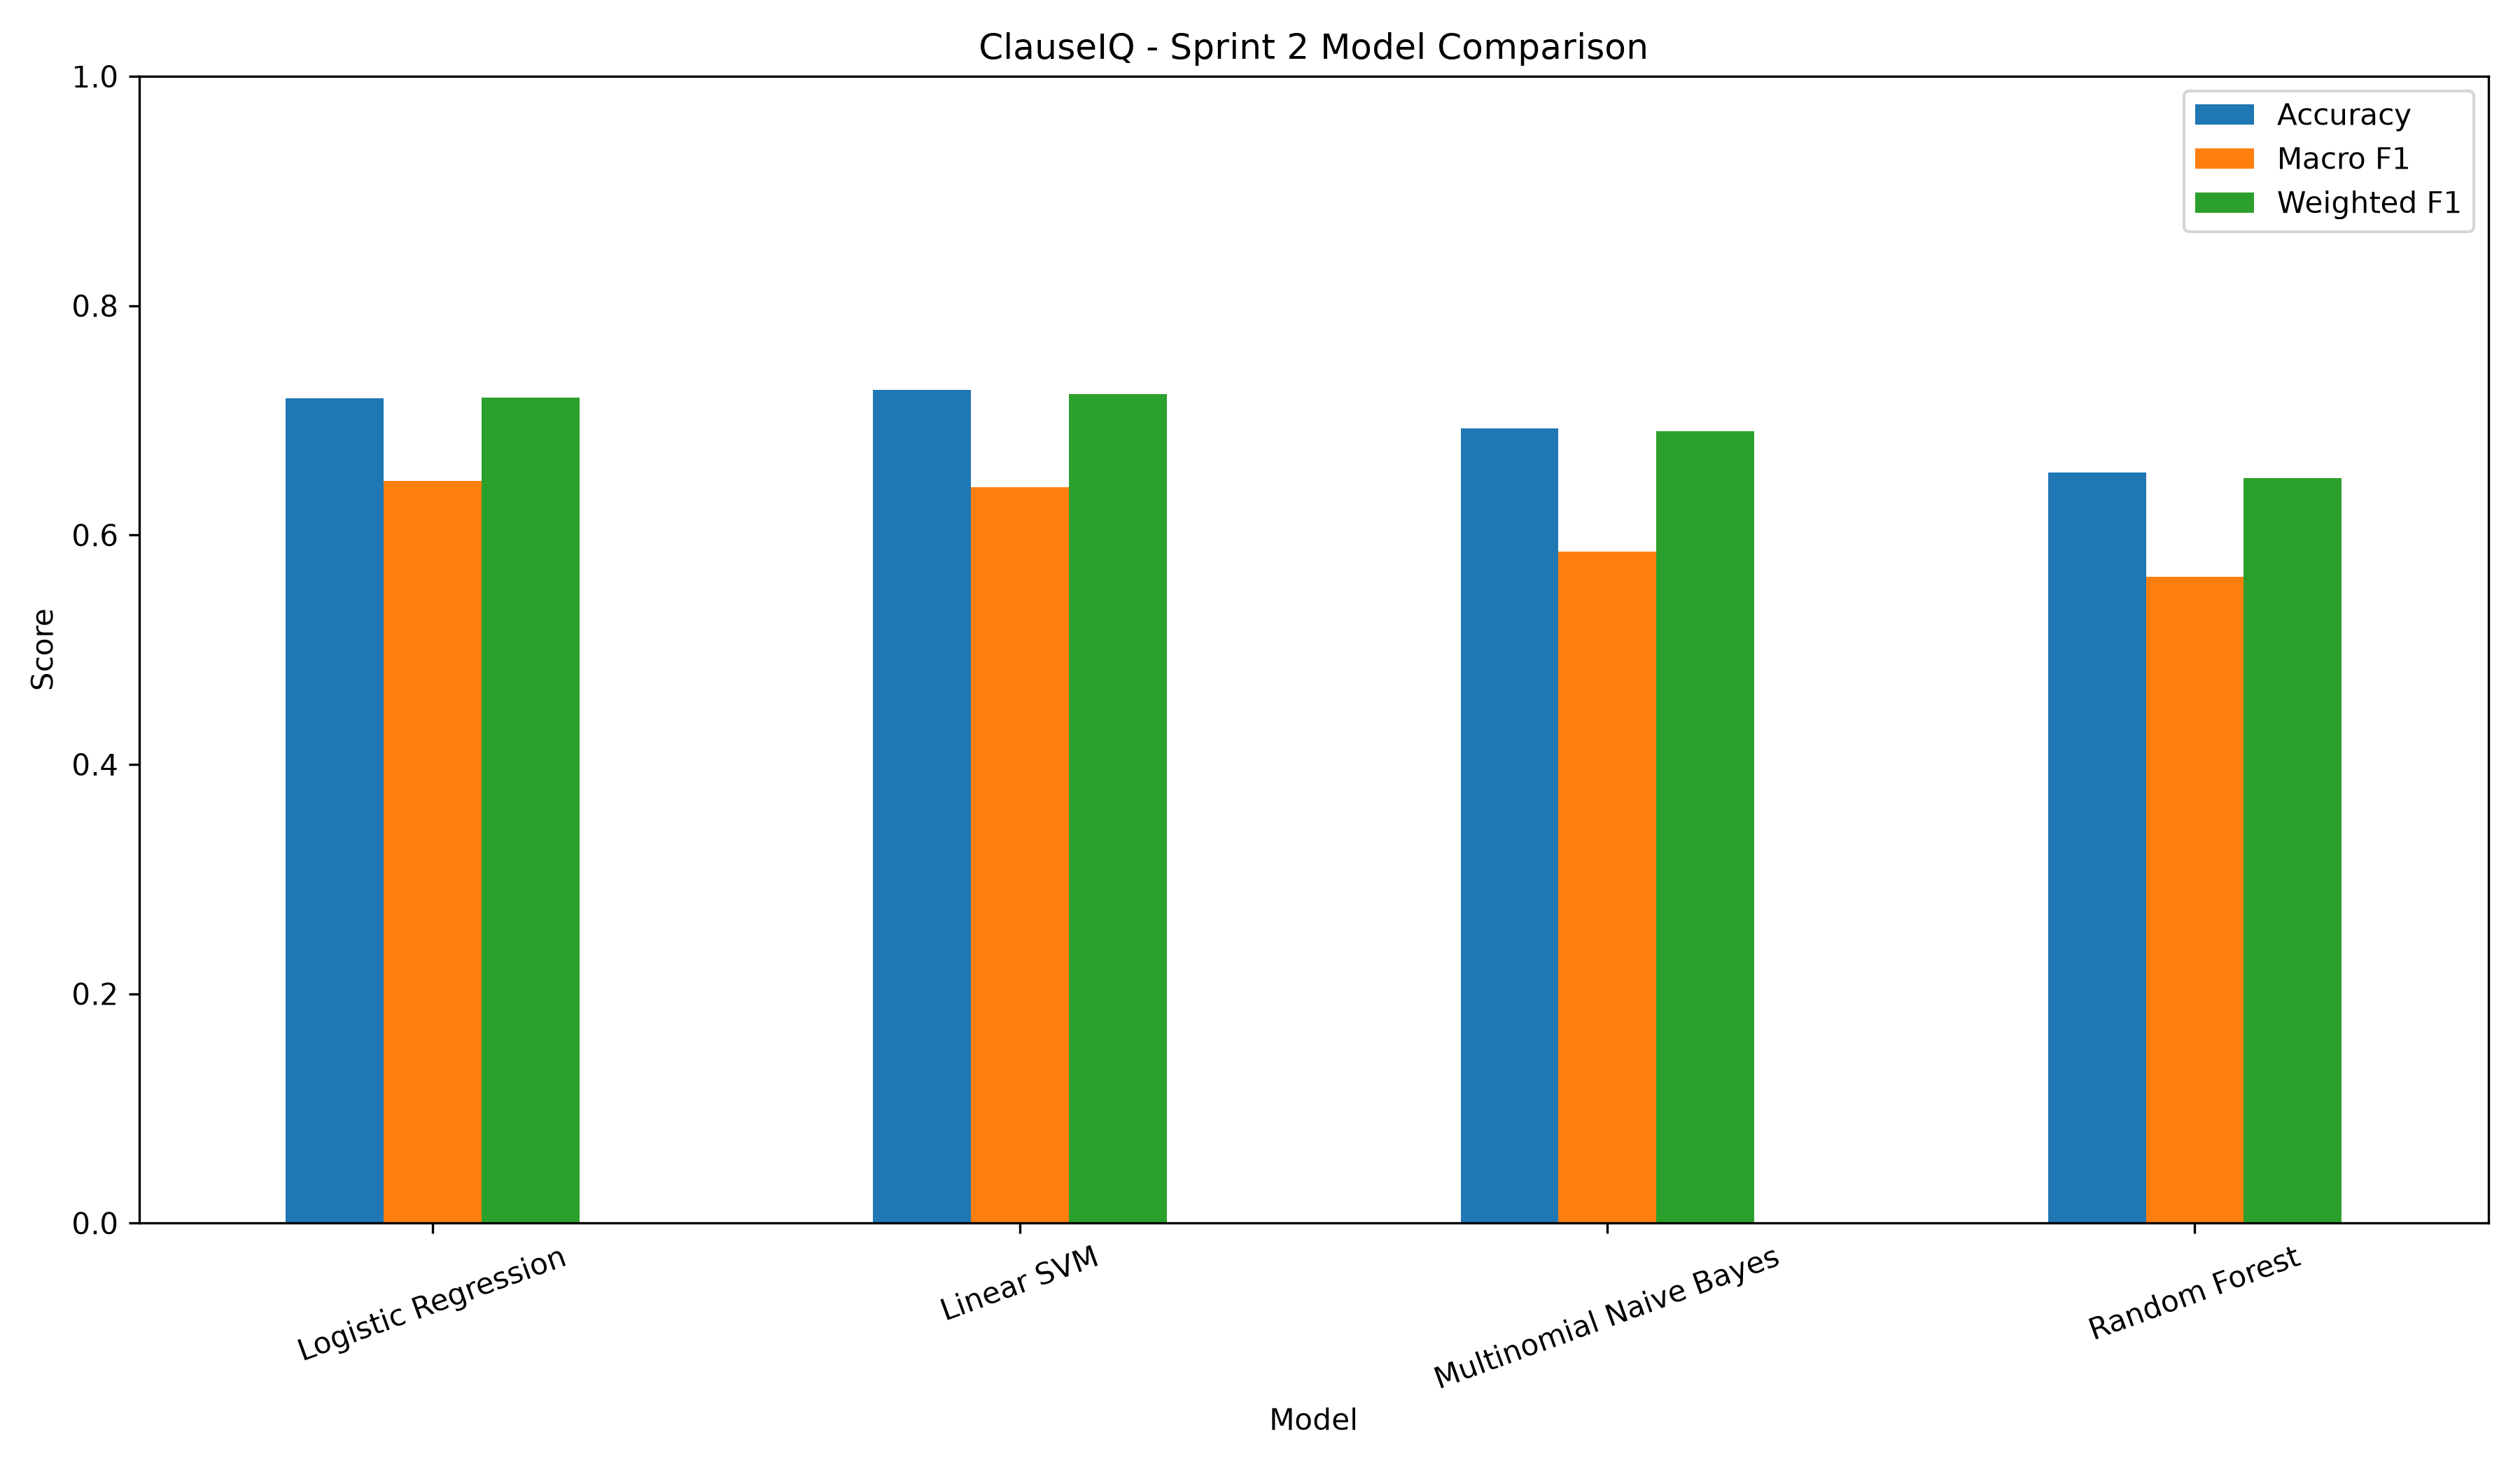
\includegraphics[width=0.88\textwidth]{figures/sprint2_model_comparison.png}
\caption{Performance comparison of the four evaluated machine learning classifiers}
\label{fig:model_comparison_chart}
\end{figure}

Figure \ref{fig:model_comparison_chart} shows that Logistic Regression and Linear SVM achieved higher overall performance than Multinomial Naive Bayes and Random Forest on the evaluated TF-IDF feature space. Linear SVM achieved the highest Accuracy of 72.63\%, while Logistic Regression achieved the highest Macro-F1 of 64.74\% and Weighted-F1 of 71.96\%. Since Macro-F1 was defined as the primary model-selection metric, Logistic Regression was selected for the ClauseIQ classification component.

% ----------------------------------------------------------------------
% Section 5.2: Evaluation Metrics
% ----------------------------------------------------------------------
\section{Evaluation Metrics}
\label{sec:evaluation_metrics}

\subsubsection*{Selection Methodology}
In accordance with the project's predefined architectural specification, model selection is governed by two hierarchical criteria:
\begin{enumerate}
    \item \textbf{Primary Selection Metric:} \textbf{Macro-Averaged F1-Score (Macro-F1)}.
    \item \textbf{Secondary Selection Metric:} \textbf{Accuracy}.
\end{enumerate}

\subsubsection*{Selected Production Classifier: Logistic Regression}
Based strictly on the primary selection criterion, \textbf{Multinomial Logistic Regression} was selected as the optimal production model for ClauseIQ:
\begin{itemize}
    \item \textbf{Logistic Regression Macro-F1:} \textbf{64.74\%} (0.6474)
    \item \textbf{Linear SVM Macro-F1:} \textbf{64.18\%} (0.6418)
    \item \textbf{Multinomial Naive Bayes Macro-F1:} \textbf{58.53\%} (0.5853)
    \item \textbf{Random Forest Macro-F1:} \textbf{56.34\%} (0.5634)
\end{itemize}

While Linear SVM achieved a marginally higher Accuracy (\textbf{72.63\%} vs. \textbf{71.90\%} for Logistic Regression), its Macro-F1 was lower by \textbf{0.56 percentage points} (64.18\% vs. 64.74\%).

\subsubsection*{Detailed Rationale for Selection}
In enterprise contract compliance, selecting an algorithm based solely on overall Accuracy is dangerously flawed. Because the CUAD corpus exhibits a 46.33:1 class imbalance, high accuracy can be achieved simply by correctly classifying ubiquitous boilerplate categories (such as \textit{Parties} with 1,251 samples or \textit{Audit Rights} with 642 samples) while failing completely on rare, highly consequential provisions. 

Minority categories—such as \textit{Price Restrictions} (27 total samples), \textit{Most Favored Nation} (42 samples), and \textit{Rofr/Rofo/Rofn} (312 samples)—carry immense commercial and legal exposure. Macro-F1 computes the unweighted arithmetic mean of F1-scores across all 41 categories, ensuring that rare, high-risk clauses receive equal optimization weight alongside high-frequency boilerplate. Logistic Regression demonstrated the highest Macro-F1 across the entire benchmark.

\subsubsection*{Conceptual Distinction Between Macro-F1 and Probability Estimates}
Macro-F1 is an aggregate classification performance metric calculated over the evaluation dataset. It is not a probability, confidence score, or indicator of the likelihood of an individual prediction. Logistic Regression provides class probability estimates through its multinomial softmax formulation. These probability estimates are distinct from the Macro-F1 evaluation metric.

% ----------------------------------------------------------------------
% Section 5.3: Confusion Matrix
% ----------------------------------------------------------------------
\section{Confusion Matrix}
\label{sec:confusion_matrix}

To analyze classification behavior across all 41 categories, full $41 \times 41$ confusion matrices were generated for all four evaluated models. Figure \ref{fig:logistic_regression_cm} presents the confusion matrix for the selected Logistic Regression model.

\begin{figure}[h!]
\centering
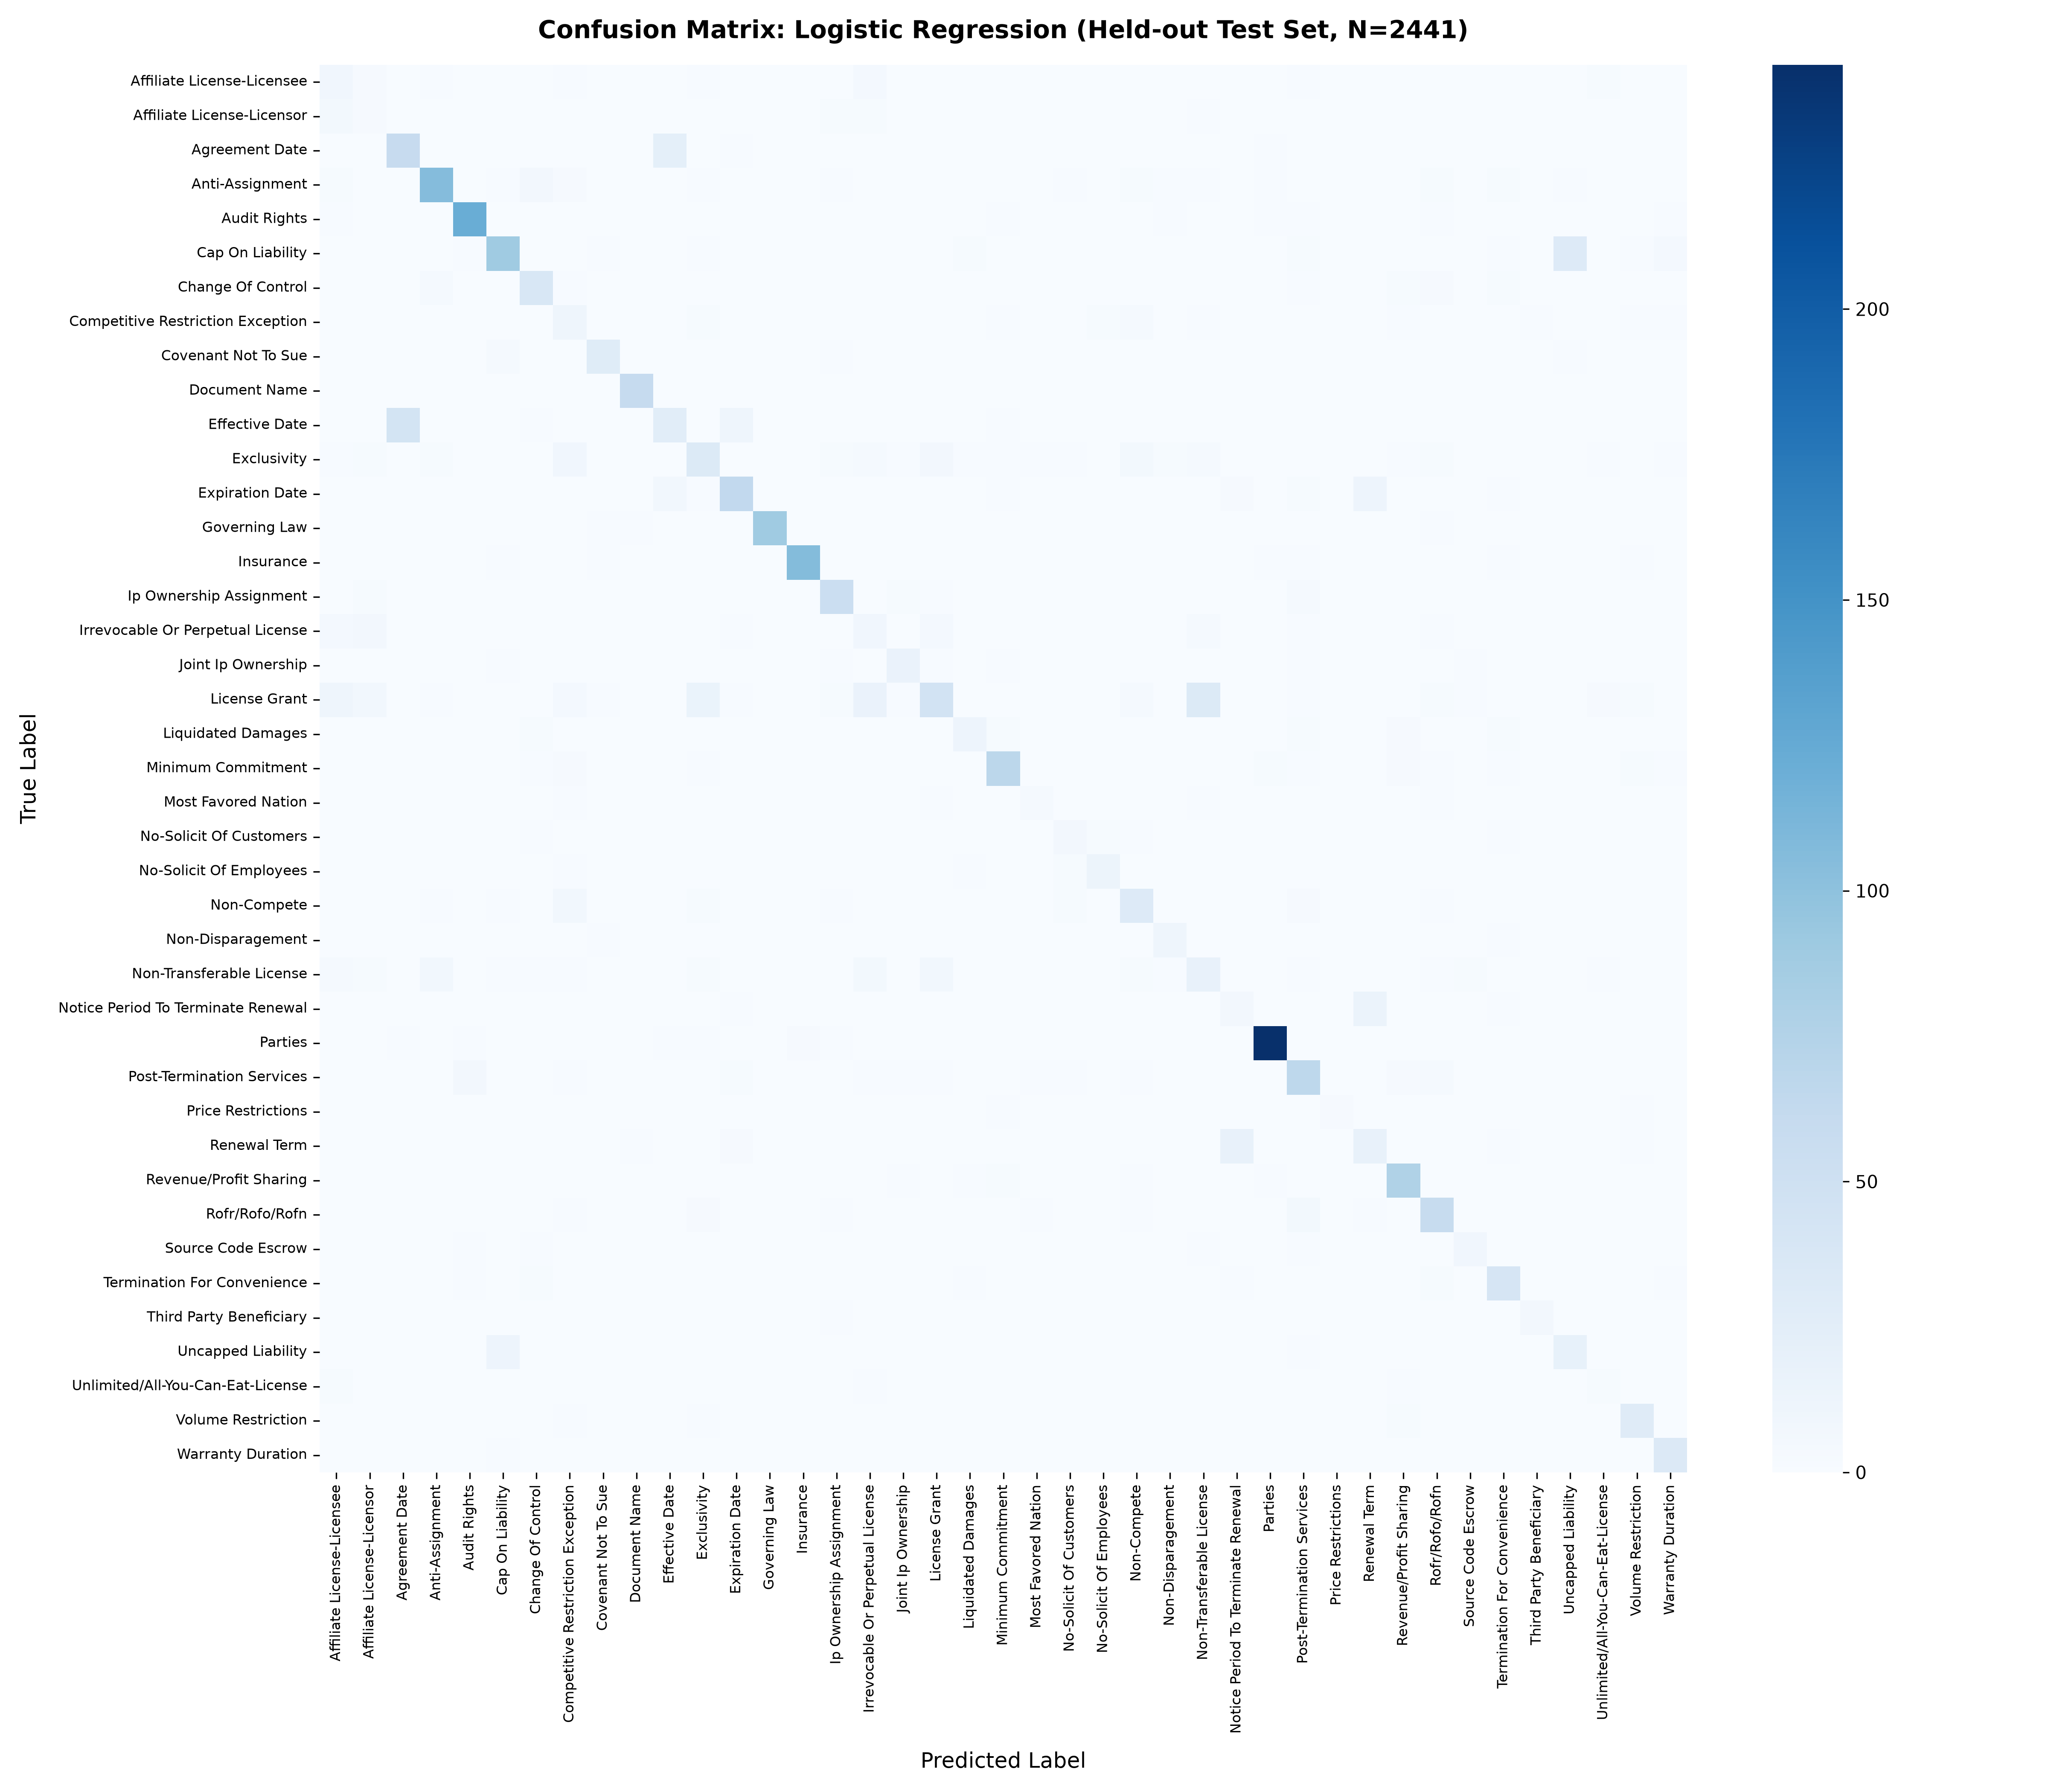
\includegraphics[width=0.92\textwidth]{figures/logistic_regression_cm.png}
\caption{Full $41 \times 41$ confusion matrix for the selected Logistic Regression model}
\label{fig:logistic_regression_cm}
\end{figure}

The confusion matrix exhibits key structural characteristics:
\begin{itemize}
    \item \textbf{Axes Definition:} The vertical axis (Y-axis) represents the True Category label, while the horizontal axis (X-axis) represents the Predicted Category label.
    \item \textbf{Diagonal Concentration:} The prominent bright diagonal represents correct classifications ($TP_c$). Strong diagonal concentration is observed across frequent legal categories, including \textit{Parties}, \textit{Audit Rights}, \textit{Governing Law}, \textit{Insurance}, and \textit{Termination For Convenience}.
    \item \textbf{Off-Diagonal Dispersion:} Off-diagonal entries denote misclassifications. Misclassifications are predominantly concentrated among semantically adjacent sub-categories:
    \begin{itemize}
        \item \textit{Affiliate License-Licensee} vs. \textit{Affiliate License-Licensor}: These classes share almost identical vocabulary regarding licensing grants, differing only in the directional party designation.
        \item \textit{Cap On Liability} vs. \textit{Uncapped Liability}: Both provisions deal with liability boundaries, often leading to mutual confusion when negative phrasing is subtle.
        \item \textit{Agreement Date} vs. \textit{Effective Date}: Both provisions contain concise calendar dates, making contextual differentiation difficult when surrounding context is absent.
    \end{itemize}
\end{itemize}

Confusion matrices for the other three evaluated architectures (\texttt{linear\_svm\_cm.png}, \texttt{multinomial\_naive\_bayes\_cm.png}, and \texttt{random\_forest\_cm.png}) demonstrate consistent diagonal patterns, with Linear SVM showing comparable sharpness to Logistic Regression, while Random Forest displays noticeable off-diagonal dispersion due to majority-class bias.

% ----------------------------------------------------------------------
% Section 5.4: Relevant Metrics Calculated from Confusion Matrix
% ----------------------------------------------------------------------
\section{Relevant Metrics Calculated from Confusion Matrix}
\label{sec:metrics_from_confusion_matrix}

From the entries of the $41 \times 41$ confusion matrix, class-specific True Positives ($TP_c$), False Positives ($FP_c$), and False Negatives ($FN_c$) are extracted to compute exact per-category Precision ($P_c = \frac{TP_c}{TP_c + FP_c}$), Recall ($R_c = \frac{TP_c}{TP_c + FN_c}$), and F1-score ($F1_c = \frac{2 P_c R_c}{P_c + R_c}$).

Table \ref{tab:representative_classes} presents representative class-level metrics derived directly from the verified confusion matrix and classification report of the selected Logistic Regression model.

\begin{table}[h!]
\centering
\small
\begin{tabular}{lcccc}
\toprule
\textbf{Category} & \textbf{Precision} & \textbf{Recall} & \textbf{F1-Score} & \textbf{Test Support} \\
\midrule
\multicolumn{5}{l}{\textbf{High-Performing Categories (Distinctive Vocabulary)}} \\
Governing Law              & 1.0000 & 0.9674 & 0.9834 & 92  \\
Parties                    & 0.9719 & 0.9680 & 0.9699 & 250 \\
Document Name              & 0.9683 & 1.0000 & 0.9839 & 61  \\
Insurance                  & 0.9725 & 0.9464 & 0.9593 & 112 \\
Audit Rights               & 0.9173 & 0.9457 & 0.9313 & 129 \\
Revenue/Profit Sharing     & 0.8280 & 0.9277 & 0.8750 & 83  \\
Termination For Convenience& 0.7455 & 0.8367 & 0.7885 & 49  \\
\midrule
\multicolumn{5}{l}{\textbf{Moderate-Performing Categories}} \\
Cap On Liability           & 0.7946 & 0.6593 & 0.7206 & 135 \\
Non-Compete                & 0.5926 & 0.6275 & 0.6095 & 51  \\
Exclusivity                & 0.5077 & 0.4024 & 0.4490 & 82  \\
Uncapped Liability         & 0.3585 & 0.5758 & 0.4419 & 33  \\
\midrule
\multicolumn{5}{l}{\textbf{Challenging / Rare Categories (Severe Imbalance)}} \\
Price Restrictions         & 1.0000 & 0.6000 & 0.7500 & 5   \\
Most Favored Nation        & 0.5714 & 0.5000 & 0.5333 & 8   \\
Affiliate License-Licensee & 0.2195 & 0.3913 & 0.2812 & 23  \\
Affiliate License-Licensor & 0.1111 & 0.2143 & 0.1463 & 14  \\
Unlimited/All-You-Can-Eat  & 0.2222 & 0.3333 & 0.2667 & 6   \\
\midrule
\textbf{Macro Average (41 Classes)}    & \textbf{0.6481} & \textbf{0.6622} & \textbf{0.6474} & \textbf{2,441} \\
\textbf{Weighted Average (41 Classes)} & \textbf{0.7354} & \textbf{0.7190} & \textbf{0.7196} & \textbf{2,441} \\
\textbf{Overall Test Accuracy}         & \multicolumn{3}{c}{\textbf{71.90\%} (0.7190)} & \textbf{2,441} \\
\bottomrule
\end{tabular}
\caption{Representative class performance for the selected Logistic Regression model}
\label{tab:representative_classes}
\end{table}

\subsubsection*{Observations on Class-Level Performance}
\begin{enumerate}
    \item \textbf{Distinctive Vocabulary Excels:} Categories characterized by standardized statutory phrasing—such as \textit{Governing Law} (F1: 98.34\%) and \textit{Insurance} (F1: 95.93\%)—achieve near-perfect classification. In \textit{Governing Law}, terms such as ``\textit{governed by}'', ``\textit{construed in accordance with}'', and specific jurisdiction names (e.g., ``\textit{Delaware}'', ``\textit{New York}'') provide decisive feature weights.
    \item \textbf{Rare Categories Maintain Viability:} Despite having only 5 test samples, \textit{Price Restrictions} achieved an F1-score of 75.00\% (100\% Precision, 60.0\% Recall), demonstrating that class-weight balancing successfully prevented the model from ignoring low-frequency classes.
    \item \textbf{Directional Ambiguity:} The lowest F1-scores occur in paired categories such as \textit{Affiliate License-Licensor} (F1: 14.63\%) and \textit{Affiliate License-Licensee} (F1: 28.12\%). Because both provisions govern software and patent grants, distinguishing the granting party from the receiving party requires fine-grained grammatical dependency parsing that bag-of-words TF-IDF representations partially compress.
\end{enumerate}

% ----------------------------------------------------------------------
% Section 5.5: Prediction Statistics of Unseen Data
% ----------------------------------------------------------------------
\section{Prediction Statistics of Unseen Data}
\label{sec:prediction_statistics_unseen}

The generalization capability of the selected Logistic Regression model was evaluated on the held-out test dataset ($N_{\text{test}} = 2,441$ unseen clauses) strictly isolated from model training. The aggregate and stratified prediction statistics across this unseen dataset are summarized below:
\begin{itemize}
    \item \textbf{Total Unseen Clauses Evaluated:} 2,441 instances.
    \item \textbf{Correct Predictions on Unseen Data:} 1,755 clauses, yielding an overall Accuracy of \textbf{71.90\%} (0.7190).
    \item \textbf{Macro-Averaged Generalization Across 41 Categories:}
    \begin{itemize}
        \item Macro Precision: \textbf{64.81\%} (0.6481)
        \item Macro Recall: \textbf{66.22\%} (0.6622)
        \item Macro-F1: \textbf{64.74\%} (0.6474)
    \end{itemize}
    \item \textbf{Weighted-Averaged Generalization Across 41 Categories:}
    \begin{itemize}
        \item Weighted Precision: \textbf{73.54\%} (0.7354)
        \item Weighted Recall: \textbf{71.90\%} (0.7190)
        \item Weighted-F1: \textbf{71.96\%} (0.7196)
    \end{itemize}
    \item \textbf{Performance by Sample Frequency Strata on Unseen Data:}
    \begin{itemize}
        \item \textit{High-Support Categories (Support $\ge 60$):} Consistently achieved $F1 > 0.85$ on unseen data (e.g., \textit{Document Name} F1: 0.9839 on 61 test clauses; \textit{Governing Law} F1: 0.9834 on 92 test clauses; \textit{Parties} F1: 0.9699 on 250 test clauses).
        \item \textit{Moderate-Support Categories ($20 \le \text{Support} < 60$):} Achieved F1 scores between 0.44 and 0.79 on unseen clauses (e.g., \textit{Termination For Convenience} F1: 0.7885 on 49 test clauses; \textit{Cap On Liability} F1: 0.7206 on 135 test clauses).
        \item \textit{Low-Support Minority Categories (Support $< 10$):} Maintained positive detection on unseen data (e.g., \textit{Price Restrictions} F1: 0.7500 on 5 test clauses; \textit{Most Favored Nation} F1: 0.5333 on 8 test clauses).
    \end{itemize}
\end{itemize}

% ----------------------------------------------------------------------
% Section 5.6: Discussion of Findings and Conclusions
% ----------------------------------------------------------------------
\section{Discussion of Findings and Conclusions}
\label{sec:discussion_of_findings}

The empirical benchmark reveals critical insights regarding algorithmic suitability for sparse legal text categorization:
\begin{enumerate}
    \item \textbf{Superiority of Linear Decision Boundaries:} Both linear architectures (Logistic Regression and Linear SVM) substantially outperformed the tree ensemble (Random Forest) and generative model (Naive Bayes). In a 10,000-dimensional sparse TF-IDF space, text data resides in an ultra-high-dimensional geometry where classes are predominantly linearly separable. Linear hyperplanes effectively integrate small weights across thousands of vocabulary terms.
    \item \textbf{Random Forest Degradation on Sparse Vectors:} Random Forest performed poorly, achieving a Macro-F1 of only 56.34\% and Accuracy of 65.46\%. In Random Forest, decision trees sample random feature subsets (typically $\sqrt{10000} = 100$ features) at each node split. In a sparse matrix where over 98\% of entries are zero, the probability of a sampled subset containing the few discriminative legal keywords is low. Consequently, individual trees often split on irrelevant noise or default to the majority class.
    \item \textbf{Naive Bayes Smoothing Constraints:} Multinomial Naive Bayes achieved respectable accuracy (69.27\%) but suffered in Macro-F1 (58.53\%). Because Naive Bayes assumes complete feature independence, strong co-occurrences in legal text (e.g., ``\textit{indemnify, defend, and hold harmless}'') violate the independence assumption, skewing class posteriors toward categories with broad vocabularies.
    \item \textbf{Conclusions on Production Model Selection:} Multinomial Logistic Regression was verified as the optimal production classifier for the ClauseIQ system. With the highest Macro-F1 score of 64.74\% across all 41 categories and balanced recall on low-frequency risk clauses, Logistic Regression provides balanced, robust categorization on real-world commercial contracts.
\end{enumerate}

% Chapters 6-10 are excluded from the Interim Report per guide structure
% (Remaining deliverables and future extensions will be documented in the Final Report)

% ------------------------------------------------------------------------------
% 10. REFERENCES
% ------------------------------------------------------------------------------
\newpage
\phantomsection
\addcontentsline{toc}{chapter}{REFERENCES}
\begin{thebibliography}{99}

\bibitem{quevedo2024}
E.~Quevedo~Caballero, T.~\v{C}ern\'{y}, A.~Rodriguez, P.~Rivas, J.~Yero, K.~Sooksatra, and D.~Taibi,
``Legal Natural Language Processing From 2015 to 2022: A Comprehensive Systematic Mapping Study of Advances and Applications,''
\textit{IEEE Access}, vol.~12, pp.~145286--145317, 2024.
\url{https://doi.org/10.1109/ACCESS.2024.3414967}

\bibitem{siino2025}
M.~Siino, M.~Falco, D.~Croce, and P.~Rosso,
``Exploring LLMs Applications in Law: A Literature Review on Current Legal NLP Approaches,''
\textit{IEEE Access}, vol.~13, pp.~18253--18276, 2025.
\url{https://doi.org/10.1109/ACCESS.2025.3533217}

\bibitem{kutbi2023}
M.~Kutbi,
``Named Entity Recognition Utilized to Enhance Text Classification While Preserving Privacy,''
\textit{IEEE Access}, vol.~11, pp.~117576--117581, 2023.
\url{https://doi.org/10.1109/ACCESS.2023.3325895}

\bibitem{cuad2021}
D.~Hendrycks, C.~Burns, A.~Chen, and S.~Ball,
``CUAD: An Expert-Annotated NLP Dataset for Legal Contract Review,''
in \textit{Proceedings of the Neural Information Processing Systems (NeurIPS)}, 2021.
\url{https://arxiv.org/abs/2103.06268}

\bibitem{scikit-learn}
F.~Pedregosa, G.~Varoquaux, A.~Gramfort, V.~Michel, B.~Thirion, O.~Grisel, M.~Blondel, P.~Prettenhofer, R.~Weiss, V.~Dubourg, J.~Vanderplas, A.~Passos, D.~Cournapeau, M.~Brucher, M.~Perrot, and E.~Duchesnay,
``Scikit-learn: Machine Learning in Python,''
\textit{Journal of Machine Learning Research}, vol.~12, pp.~2825--2830, 2011.

\bibitem{spacy2017}
M.~Honnibal and I.~Montani,
``spaCy: Industrial-strength Natural Language Processing in Python,''
\textit{Zenodo}, 2017.

\bibitem{fastapi}
S.~Ram\'irez,
``FastAPI: High performance, easy to learn, fast to code, ready for production,''
2018. \url{https://fastapi.tiangolo.com/}

\end{thebibliography}

\end{document}
